%\newcommand{\CLASSINPUTinnersidemargin}{0.7in}
%\newcommand{\CLASSINPUToutersidemargin}{0.7in}

\documentclass{article}

\usepackage{fullpage} % use entire page layout
\usepackage{times}     % smaller and better fonts that the standard latex ones
\usepackage[letterpaper]{geometry} % force letter format
\usepackage[colorlinks=true,linkcolor=black,urlcolor=blue,anchorcolor=black,citecolor=black,backref=none]{hyperref}
\usepackage[usenames,dvipsnames]{color}
%% Disable backref and make \href colors more decent:
\definecolor{MyDarkBlue}{rgb}{0,0.1,0.7}
\hypersetup{pdfborder={0 0 0},colorlinks,breaklinks=true,
  urlcolor={MyDarkBlue},citecolor={MyDarkBlue},linkcolor={MyDarkBlue} }
\newcommand{\ebookurl}{http://www.sigcomm.org/content/ebook}

\usepackage[absolute,showboxes]{textpos}

%set unit to be pagewidth and height, and increase inner margin of box
\setlength{\TPHorizModule}{\paperwidth}
\setlength{\TPVertModule}{\paperheight}
\TPMargin{5pt}

%define \copyrightstatement command for easier use
\newcommand{\copyrightstatement}{
    \begin{textblock}{0.65}(0.17,0.9)    % tweak here: {box width}(hposition, vposition)
         \noindent
         \footnotesize
         J. Cordero, J. Yi, T. Clausen, E. Baccelli ``Enabling Multihop Communication in Spontaneous Wireless Networks'', in H. Haddadi, O. Bonaventure (Eds.), \href{\ebookurl}{\emph{Recent
         Advances in Networking}}, (2013), pp. 413-457. Licensed under a
         \href{http://creativecommons.org/licenses/by-sa/3.0/}{CC-BY-SA}
         Creative Commons license. 
    \end{textblock}
}

\usepackage{graphicx}
\usepackage{multirow}
\usepackage{array}
\usepackage{fancyvrb}
\usepackage{boxedminipage}
\usepackage{color}
\usepackage{paralist}
\usepackage{algorithmic}
\usepackage{slashbox}
\usepackage{xspace}
\usepackage{url}
\usepackage{subfig}
\usepackage{amsthm}
\newcommand{\ed}[1]{\textsf{\textcolor{red}{[#1]}}}
\newcommand{\remove}[1]{}
\usepackage{epstopdf}
\epstopdfsetup{update}

\title{Recent Advances in Reliable Transport Protocols\footnote{
Parts of the text in this chapter have appeared in the following
 publications by the same author(s): \cite{login}, \cite{mptcp-cc},
 \cite{raiciu2012hard}, ~\cite{nowlan12fitting} 
and~\cite{iyengar10minion}.}
}

\author{Costin Raiciu, Janardhan Iyengar, Olivier Bonaventure}

\date{}



\begin{document}

\pagestyle{empty}

\maketitle

\thispagestyle{empty}

\begin{abstract}
Transport protocols play a critical role in today's Internet. This
chapter first looks at the recent of the reliable transport
protocols. It then explains the growing impact of middleboxes on the
evolvability of these protocols. 
Two recent protocol extensions,
Multipath TCP and Minion,
which were both designed to extend the current Transport Layer 
in the Internet
are then described.
\end{abstract}


\section{Introduction}
%%%%%%%%%%%%%%%%%%

Professors often rely on textbooks to teach undergraduate and graduate networking courses. While there are many good introductory textbooks, there are very few books on advanced networking topics that could be suitable to graduate courses in networking. To fill this gap, SIGCOMM Education Committee has launched a community project to develop a high-quality, open-source, edited eBook on �Recent Advances in Networking�. This eBook will be distributed online via the SIGCOMM website. 

This eBook is composed of nine chapters chosen after a highly selective review process by the editorial board. The selected chapters cover advanced networking topics and accompanying teaching material (slides and exercises). All the source code of the eBook and the teaching material are kept on a version controlled repository that will be accessible for the entire SIGCOMM community. We expect that releasing such high quality teaching material will be beneficial for a large number of students and professors. The teaching material will be updated on a regular basis to reflect new advances in our field. We will also be adding new chapters on more emerging topics in the future volumes.


We wish to thank all there authors for providing such high quality chapters. We are also grateful to the reviewers and the editorial board for spending many hours on each chapter to ensure a coherent level amongst all the chapters. We hope you enjoy reading this eBook and find it a useful resource.

Hamed Haddadi, Olivier Bonaventure

August 2013


\section{Today's Internet}\label{section:today}
%%%%%%%%%%%%%%%%%%%%%


The TCP/IP protocol suite was designed with the end-to-end principle \cite{saltzer1984end} in mind. TCP and SCTP are no exception to this rule. They both assume that the network contains relays that operate only at the physical, datalink and network layers of the reference models. 

In such an end-to-end Internet, the payload of an IP packet is never modified inside the network and any transport protocol can be used above IPv4 or IPv6. Today, this behavior corresponds to some islands in the Internet like research backbones and some university networks. Measurements performed in enterprise, cellular and other types of commercial networks reveal that IP packets are processed differently in deployed networks \cite{honda2011still,wang2011untold}.

In addition to the classical repeaters, switches and routers, currently deployed networks contain various types of middleboxes \cite{rfc3234}.  Middleboxes were not part of the original TCP/IP architecture and they have evolved mainly during the last decade. A recent survey in enterprise networks reveals that such networks contain sometimes as many middleboxes as routers \cite{sherry2012making}. 

A detailed survey of all possible middleboxes is outside the scope of this chapter, but it is useful to study the operation of some important types of middleboxes to understand their impact on transport protocols and how transport protocols have to cope with them. 

\subsection{Firewalls}

Firewalls perform checks on the received packets and decide to accept or discard them based on configured security policies. Firewalls play an important role in delimiting network boundaries and controlling incoming and outgoing traffic in enterprise networks. In theory, firewalls should not directly affect transport protocols, but in practice, they may block the deployment of new protocols or extensions to existing ones. Firewalls can either filter packets on the basis of a white list, i.e. an explicit list of allowed communication flows, or a black list, i.e. an explicit list of all forbidden communication flows. Most enterprise firewalls use a white list approach. The network administrator defines a set of allowed communication flows, based on the high-level security policies of the enterprise and configures the low-level filtering rules of the firewall to implement these policies. With such a whitelist, all flows that have not been explicitly defined are forbidden and the firewall discards all packets that do not match an accepted communication flow. This unfortunately implies that a packet that contains a different \emph{Protocol} than the classical TCP, ICMP and UDP protocols will usually not be accepted by such a firewall. This is a major hurdle for the deployment of new transport protocols like SCTP. 

Some firewalls can perform more detailed verification and maintain state for each established TCP connection. Some of these stateful firewalls are capable of verifying whether a packet that arrives for an accepted TCP connection contains a valid sequence number. For this, the firewall maintains state for each TCP connection that it accepts and when a new data packet arrives, it verifies that it belongs to an established connection and that its sequence number fits inside the advertised receive window. This verification is intended to protect the hosts that reside behind the firewall from packet injection attacks despite the fact that these hosts also need to perform the same verification. 

Stateful firewalls may also limit the extensibility of protocols like TCP. To understand the problem, let us consider the large windows extension defined in \cite{rfc1323}. This extension fixes one limitation of the original TCP specification. The TCP header \cite{rfc793} includes a 16-bits field that encodes the receive window in the TCP header. A consequence of this choice is that the standard TCP cannot support a receive window larger than 64 KBytes. This is not large enough for high bandwidth networks. To allow hosts to use a larger window, \cite{rfc1323} changes the semantics of the \emph {receive window} field of the TCP header on a per-connection basis. \cite{rfc1323} defines the \texttt{WScale} TCP option that can only be used inside the \texttt{SYN} and \texttt{SYN+ACK} segments. This extension allows the communicating hosts to maintain their receive window as a 32 bits field. The \texttt{WScale} option contains as parameter the number of bits that will be used to shift the 32-bits window to the right before placing the lower 16 bits in the TCP header. This shift is used on a TCP connection provided that both the client and the server have included the \texttt{WScale} option in the \texttt{SYN} and \texttt{SYN+ACK} segments.

Unfortunately, a stateful firewall that does not understand the \texttt{WScale} option, may cause problems. Consider for example a client and a server that use a very large window. During the three-way handshake, they indicate with the \texttt{WScale} option that they will shift their window by $14$ bits to the right. When the connection starts, each host reserves $2^{17}$ bytes of memory for its receive window\footnote{It is common to start a TCP connection with a small receive window/buffer and automatically increase the buffer size during the transfer \cite{Semke:1998hf}.}. Given the negotiated shift, each host will send in the TCP header a window field set to \texttt{0000000000000100}. If the stateful firewall does understand the \texttt{WScale} option used in the \texttt{SYN} and \texttt{SYN+ACK} segments, it will assume a window of 4 bytes and will discard all received segments. Unfortunately, there are still today stateful firewalls\footnote{See e.g. \url{http://support.microsoft.com/kb/934430}} that do not understand this TCP option defined in 1992.

Stateful firewalls can perform more detailed verification of the packets exchanged during a TCP connection. For example, intrusion detection and intrusion prevention systems are often combined with traffic normalizers \cite{Vutukuru_TCP:2008,handley2001network}. A traffic normalizer is a middlebox that verifies that all packets obey the protocol specification. When used upstream of an intrusion detection system, a traffic normalizer can for example buffer the packets that are received out-of-order and forward them to the IDS once they are in-sequence.

\subsection{Network Address Translators}

A second, and widely deployed middlebox, is the Network Address Translator (NAT). The NAT was defined in \cite{rfc1631} and various extensions have been developed over the years. One of the initial motivation for NAT was to preserve public IP addresses and allow a group of users to share a single IP address. This enabled the deployment of many networks that use so-called \emph{private addresses} \cite{rfc1918} internally and rely on NATs to reach the global Internet. At some point, it was expected that the deployment of IPv6 would render NAT obsolete. This never happened and IPv6 deployment is still very slow \cite{Dhamdhere_IPv6:2012}. Furthermore, some network administrators have perceived several benefits with the deployment of NATs \cite{rfc2993} including : reducing the exposure of addresses, topology hiding, independence from providers, \ldots Some of these perceived advantages have caused the IETF to consider NAT for IPv6 as well, despite the available address space. Furthermore, the IETF, vendors and operators are considering the deployment of large scale Carrier Grade NATs (CGN) to continue to use IPv4 despite the depletion of the addressing space \cite{Perreault_CGN:2012} and also to ease the deployment of IPv6 \cite{rfc6264}. NATs will remain a key element of the deployed networks for the foreseeable future. 

There are different types of NATs depending on the number of addresses that they support and how they maintain state. In this section, we concentrate on a simple but widely deployed NAT that serves a large number of users on a LAN and uses a single public IP address. In this case, the NAT needs to map several private IP addresses on a single public address. To perform this translation and still allow several internal hosts to communicate simultaneously, the NAT must understand the transport protocol that is used by the internal hosts. For TCP, the NAT needs to maintain a pool of TCP port numbers and use one of the available port as the source port for each new connection initiated by an internal host. Upon reception of a packet, the NAT needs to update the source and destination addresses, the source (or destination) port number and also the IP and TCP checksums. The NAT performs this modification transparently in both directions. It is important to note that a NAT can only change the header of the transport protocol that it supports. Most deployed NATs only support TCP \cite{rfc5382}, UDP \cite{rfc4787} and ICMP \cite{rfc5508}. Supporting another transport protocol on a NAT requires software changes \cite{Hayes_NAT:2008} and few NAT vendors implement those changes. This often forces users of new transport protocol to tunnel their protocol on top of UDP to traverse NATs and other middleboxes \cite{rfc6773,Tuexen_Encap:2013}. This limits the ability to innovate in the transport layer.

NAT can be used transparently by most Internet applications. Unfortunately, some applications cannot easily be used over NATs \cite{rfc3027}. The textbook example of this problem is the File Transfer Protocol (FTP) \cite{rfc959}. An FTP client uses two types of TCP connections : a control connection and data connections. The control connection is used to send commands to the server. One of these is the \texttt{PORT} command that allows to specify the IP address and the port numbers that will be used for the data connection to transfer a file. The parameters of the \texttt{PORT} command are sent using a special ASCII syntax \cite{rfc959}. To preserve the operation of the FTP protocol, a NAT can translate the IP addresses and ports that appear in the IP and TCP headers, but also as parameters of the \texttt{PORT} command exchanged over the data connection. Many deployed NATs include Application Level Gateways (ALG) \cite{rfc3027} that implement part of the application level protocol and modify the payload of segments. For FTP, after translation a \texttt{PORT} command may be longer or shorter than the original one. This implies that the FTP ALG needs to maintain state and will have to modify the sequence/acknowledgment numbers of all segments sent over a connection after having translated a \texttt{PORT} command. This is transparent for the FTP application, but has influenced the design of Multipath TCP although recent FTP implementations rarely use the \texttt{PORT} command\cite{rfc2428}.

\subsection{Proxies}

The last middlebox that we cover is the proxy. A proxy is a middlebox that resides on a path and terminates TCP connections. A proxy can be explicit or transparent. The SOCKS5 protocol \cite{rfc1928} is an example of the utilization of an explicit proxy. SOCKS5 proxies are often used in enterprise networks to authenticate the establishment of TCP connections. A classical example of transparent proxies are the HTTP proxies that are deployed in various commercial networks to cache and speedup HTTP requests. In this case, some routers in the network are configured to intercept the TCP connections and redirect them to a proxy server \cite{McLaggan_WCCP:2012}. This redirection is transparent for the application, but from a transport viewpoint, the proxy acts as a relay between the two communicating hosts and there are two different TCP connections\footnote{Some deployments use several proxies in cascade. This allows the utilization of compression techniques and other non-standard TCP extensions on the connection between two proxies.}. The first one is initiated by the client and terminates at the proxy. The second one is initiated by the proxy and terminates at the server. The data exchanged over the first connection is passed to the second one, but the TCP options are not necessarily preserved. In some deployments, the proxy can use different options than the client and/or the server.


\subsection{How prevalent are middleboxes?}

We've learnt that middleboxes of various kinds exist, but are they really deployed in today's networks? Answering
this question can guide the right way to develop new protocols and enhance existing ones. 

Here we briefly review measurement studies that have attempted to paint an accurate image of middlebox
deployments in use. The conclusion is that middleboxes are widespread to the point where 
end-to-end paths without middleboxes have become exceptions, rather than the norm.

There are two broad types of middlebox studies.
The first type of study uses ground-truth topology information from providers and other organizations.
While accurate, these studies may overestimate the influence of middleboxes on end-to-end traffic because
certain behavior is only triggered in rare, corner cases (e.g. an intrusion prevention system may only affect
traffic carrying known worm signatures). These studies do not tell us exactly \emph{what operations} are applied
to packets by middleboxes.
One recent survey study has found that the 57 enterprise networks surveyed deploy as many 
middleboxes as routers \cite{sherry2012making}. 

Active measurements probe end-to-end paths to trigger ``known'' behaviors of middleboxes.
Such measurements are very accurate, pinpointing exactly what middleboxes do in certain scenarios.
However, they offer a lower bound of middlebox deployments, as they may pass through other 
middleboxes without triggering them. Additionally, such studies are limited to
probing a full path (cannot probe path segments) thus cannot tell how many middleboxes are deployed 
on a path exhibiting middlebox behavior. The data surveyed below comes from such studies. 

Network Address Translators are easy to test for: the traffic source needs to compare its local source address
with the source address of its packets reaching an external site (e.g. what's my IP). When the addresses differ,
a NAT has been deployed on path. Using this basic technique, existing studies have shown that NATs are deployed almost
universally by (or for) end-users, be they home or mobile:
\begin{itemize}
\item Most cellular providers use them to cope with address space shortage and to provide some level of security. A study surveying 107
cellular networks across the globe found that 82 of them used NATs \cite{wang2011untold}.
\item Home users receive a single public IP address (perhaps via DHCP) from their access providers, and deploy NATs to support
multiple devices. The typical middlebox here is the ``wireless router'', an access point that aggregates all home traffic 
onto the access link. A study using peer-to-peer clients found that only 12\% of the peers have a public IP address \cite{nat-study}.
\end{itemize}

Testing for stateless firewalls is equally simple: the client generates traffic using different transport protocols and port
numbers, and the server acks it back. As long as some tests work, the client knows the endpoint is reachable, and that the failed
tests are most likely due to firewall behavior. There is a chance that the failed tests are due to the stochastic packet loss
inherent in the Internet; that is why tests are interleaved and run multiple times.

Firewalls are equally widespread in the Internet, being deployed by most cellular operators \cite{netpiculet}. Home routers often act as
firewalls, blocking new protocols and even existing ones (e.g. UDP) \cite{nat-study}. Most servers also deploy firewalls to restrict
in-bound traffic \cite{sherry2012making}. Additionally, many modern operating systems come with ``default-on'' firewalls. For instance, 
the Windows 7 firewall explicitly asks users to allow incoming connections and to whitelist applications allowed to make outgoing 
connections.

Testing for explicit proxies can be done by comparing the segments that leave the source with the ones arriving at the destination.
A proxy will change sequence numbers, perhaps segment packets differently, modify the receive window, and so forth. Volunteers 
from various parts of the globe ran TCPExposure, a tool that aims to detect such proxies and other middlebox behavior 
\cite{honda2011still}. The tests cover 142 access networks (including cellular, DSL, public hotspots and offices) in 
24 countries. Proxying behavior was seen on 10\% of the tested paths\cite{honda2011still}. 

Beyond basic reachability, middleboxes such as traffic normalizers and stateful firewalls have some expectations on the packets they see: what exactly do these middleboxes do, and how widespread are they? The same study sheds some light into
this matter:
\begin{itemize}
\item Middlebox behavior depends on the ports used. Most middleboxes are active on port 80 (HTTP traffic).
\item A third of paths keep TCP flow state and use it to actively correct acknowledgments for data the middlebox has not
seen. To probe this behavior, TCPExposure sends a few TCP segments leaving a gap in the sequence number, while the server
acknowledgment also covers the gap. 
\item 14\% of paths remove unknown options from SYN packets. These paths will not allow TCP extensions to be deployed.
\item 18\% of paths modify sequence numbers; of these, a third seem to be proxies, and the other are most likely
firewalls than randomize the initial sequence number to protect vulnerable end hosts against in-window injection attacks.
\end{itemize}
 

\subsection{The Internet is Ossified}

Deploying a new IP protocol requires a lot of investment to change all the deployed hardware. Experience
with IPv6 after 15 years since it has been standardized is not encouraging: only a minute fraction of the Internet has
migrated to v6, and there are no signs of it becoming ``the Internet'' anytime soon. 

Changing IPv4 itself is in theory possible with IP options. Unfortunately, it has been known for a while now
that ``IP options are not an option'' \cite{fonseca2005ip}. This is because existing routers implement forwarding in hardware 
for efficiency reasons; packets carrying unknown IP options are treated as exceptions that are processed in software.
To avoid a denial-of-service on routers' CPU's, such packets are dropped by most routers. 

In a nutshell, we can't really touch IP - but have we also lost our ability to change transport protocols as well? 
The high level picture emerging from existing middlebox studies is that of a network that is highly tailored to today's traffic
to the point it is ossified: \emph{changing existing transport protocols is challenging as it needs to carefully consider
middlebox interactions}. Further, \emph{deploying new transport protocols natively is almost impossible}. 

Luckily, changing transport protocols is still possible, albeit great care must be taken when doing so. 
Firewalls will block \emph{any} traffic they do not understand, so deploying new protocols
must necessarily use existing ones just to get through the network. This observation has recently lead to the development
of Minion, a container protocol that enables basic connectivity above TCP while avoiding its in-order, reliable bytestream
semantics at the expense of slightly increased bandwidth usage. We discuss Minion in Section \ref{section:minion}.

Even changing TCP is very difficult. The semantics of TCP are embedded in the network fabric, and new extensions
must function within the confines of these semantics, or they will fail. In section \ref{section:mptcp} we discuss Multipath TCP, 
another recent extension to TCP, that was designed explicitly to be middlebox compatible.  



%\section{Structuring the transport layer}
%%%%%%%%%%%%%%%%%%%%%%%%%%%%%%%%%%

%\ed{Part III shows how TCP's mechanisms can be decomposed into separate layers, and this helps us understand which parts are de-facto fixed in any new transport for the new transport to remain network-compatible, and which parts can be evolved. \textbf{Jana - 5-6 pages}}

\ed{Jana, if you cannot deliver this part, please remove the section}

\section{Multipath TCP}\label{section:mptcp}

%%%%%%%%%%%%%%%%%%%%


%\ed{> Part IV describes in great detail Multipath TCP and TCP Minion,
%two recent significant evolutions of TCP that were built with
%deployability in mind. \textbf{Multipath TCP - Costin (10 pages)}}

Today's networks are multipath: mobile devices have multiple wireless
interfaces, datacenters have many redundant paths between servers and
multi-homing has become the norm for big server farms. Meanwhile, TCP
is essentially a single path protocol: when a TCP connection is
established, it is bound to the IP addresses of the two communicating
hosts. If one of these addresses changes, for whatever reason, the
connection fails. In fact a TCP connection cannot even be
load-balanced across more than one path within the network, because
this results in packet reordering and TCP misinterprets this
reordering as congestion and slows down.

This mismatch between today's multipath networks and TCP's single-path
design creates tangible problems. For instance, if a smartphone's WiFi interface
loses signal, the TCP connections associated with it stall - there is
no way to migrate them to other working interfaces, such as 3G. This
makes mobility a frustrating experience for users.  Modern datacenters
are another example: many paths are available between two endpoints,
and equal cost multipath routing randomly picks one for a particular TCP
connection.  This can cause collisions where multiple flows get placed
on the same link, hurting throughput - to such an extent that average 
throughput is halved in some scenarios.

Multipath TCP (MPTCP) \cite{rfc6284} is a major modification to TCP that allows multiple
paths to be used simultaneously by a single 
connection. Multipath TCP circumvents the issues above and several
others that affect TCP.  Changing TCP to use multiple paths is not a
new idea: it was originally proposed more than fifteen years ago by
Christian Huitema in the Internet Engineering Task Force (IETF) \cite{Huitema_Multi-homed:1995}, and
there have been a half-dozen more proposals since then to similar
effect. Multipath TCP draws on the experience gathered in previous
work, and goes further to solve issues of fairness when competing with
regular TCP and deployment issues due to middleboxes in today's
Internet. 

\subsection{Overview of Multipath TCP}

The design of Multipath TCP has been influenced by many requirements,
but there are two that stand out: application compatibility and
network compatibility. Application compatibility implies that 
applications that today run over TCP should work without any change 
over Multipath TCP. Next, Multipath TCP must
operate over any Internet path where the TCP protocol operates.

As explained earlier, many paths on today's Internet include middleboxes that, unlike routers,
 know about the TCP connections they forward, and affect them in special ways. 
Designing TCP extensions that can safely traverse all these middleboxes has
proven to be challenging.

Multipath TCP allows multiple "subflows" to be combined to form a single MPTCP
session.  An MPTCP session starts with an initial subflow which is
very similar to a regular TCP connection, with a three way handshake.  After
the first MPTCP subflow is set up, additional subflows can be
established.  Each subflow also looks very similar to a
regular TCP connection, complete with three-way handshake and graceful tear-down,
but rather than being a separate connection it is bound into an
existing MPTCP session.  Data for the connection can
then be sent over any of the active subflows that has the capacity to
take it.

To examine Multipath TCP in more detail, let us consider a very simple
scenario with a smartphone client and a single-homed server. The
smartphone has two network interfaces: a WiFi interface and a 3G
interface; each has its own IP address.  The server, being
single-homed, has a single IP address. In this environment, Multipath
TCP would allow an application on the mobile device to use a single MPTCP
session that can use both the WiFi and the 3G interfaces to
communicate with the server.  The application opens a regular TCP socket, and
the kernel enables MPTCP by default if the remote end supports it, using both paths. 
The application does not need to concern itself with which radio interface is working best at any instant;
MPTCP handles that for it. In fact, Multipath TCP can work when
both endpoints are multihomed (in this case subflows are opened between
all pairs of "compatible" IP addresses), or even in the case when 
both endpoints are single homed (in this case different subflows will use
 different port numbers, and can be routed differently by multipath routing 
in the network). 

\paragraph{Connection Setup.} Let us walk through the establishment of an MPTCP connection. 
Assume that the mobile device chooses its 3G interface to open the
connection. It first sends a \texttt{SYN} segment to the server. This segment
contains the \texttt{MP\_CAPABLE} TCP option indicating that the mobile device
supports Multipath TCP. This option also contains a key which is
chosen by the mobile device. The server replies with a \texttt{SYN+ACK} segment
containing the \texttt{MP\_CAPABLE} option and the key chosen by the server. The
mobile device completes the handshake by sending an \texttt{ACK} segment.

The initial MPTCP connection setup is shown graphically in the top part of Figure \ref{fig:mptcp_handshake},
where the segments are regular TCP segments carrying new multipath TCP-related options (shown in green).

\begin{figure}[t]
\centering
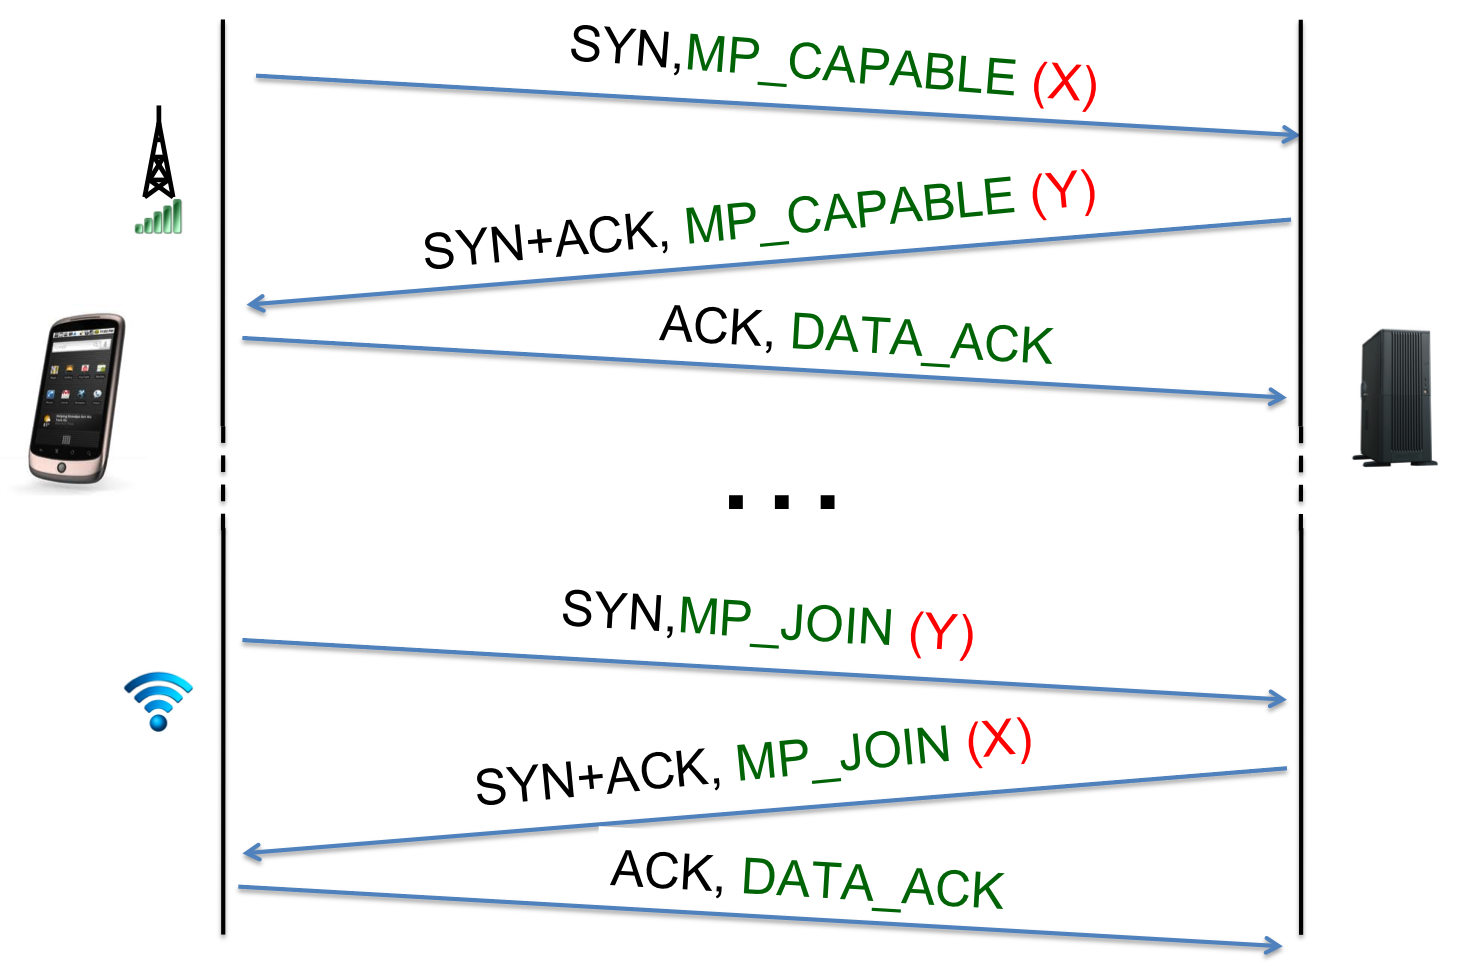
\includegraphics[width=0.9\textwidth]{figures/mptcp_handshake.png}
\caption{Multipath TCP handshake: multiple subflows can be added and removed after the initial
connection is setup and connection identifiers are exchanged.}
\label{fig:mptcp_handshake}
\end{figure}

At this point the Multipath TCP connection is established and the
client and server can exchange TCP segments via the 3G path. How
could the mobile device also send data through this Multipath TCP
session over its WiFi interface?

Naively, it could simply send some of the segments over the WiFi
interface.  However most ISPs will drop these packets, as they would
have the source address of the 3G interface.  Perhaps the client could
tell the server the IP address of the WiFi interface, and use that
when it sends over WiFi?  Unfortunately this will rarely work:
firewalls and similar stateful middleboxes on the WiFi path expect to
see a \texttt{SYN} segment before they see data segment.  The only solution that
will work reliably is to perform a regular three-way handshake on the WiFi path
before sending any packets that way, so this is what Multipath TCP
does.  This handshake carries the \texttt{MP\_JOIN} TCP option, providing
information to the server that can securely identify the
correct connection to associate this additional subflow with.  The
server replies with \texttt{MP\_JOIN} in the \texttt{SYN+ACK}, and the new subflow is
established (this is shown in the bottom part of Figure \ref{fig:mptcp_handshake}). 

An important point about Multipath TCP, especially in the context of 
mobile devices, is that the set of subflows that are associated to a Multipath TCP 
connection is not fixed. Subflows can be dynamically added and removed from a 
Multipath TCP connection throughout its lifetime, without affecting the 
bytestream transported on behalf of the application. 
If the mobile device moves to another WiFi network, it will receive a new IP 
address. At that time, it will open a new subflow using its newly allocated address 
and tell the server that its old address is not usable anymore. The server will now 
send data towards the new address. These options allow mobile devices to easily move
through different wireless connections without breaking their
Multipath TCP connections \cite{Paasch_Mobile:2012}.

Multipath TCP also implements mechanisms that allows to inform the
remote host of the addition/removal of addresses even when an endpoint operates behind a NAT, or when a subflow using a
different address family is needed (e.g. IPv6). Endpoints can send
an \texttt{ADD\_ADDR} option that contains an address identifier together with an address.
The address identifier is unique at the sender, and allows it to identify its addresses
even when it is behind a NAT. Upon receiving an advertisement, the endpoint may initiate a new subflow to
the new address. An address withdrawal mechanism is also provided via the \texttt{REMOVE\_ADDR}
option that also carries an address identifier. 

\paragraph{Data Transfer.} Assume now that two subflows have been established over WiFi and 3G:
the mobile device can send and receive data segments over both. Just like TCP, Multipath
TCP provides a bytestream service to the application.  In
fact, standard applications can function over MPTCP without being
aware of it - MPTCP provides the same socket interface as TCP.

Since the two paths will often have different delay characteristics,
the data segments sent over the two subflows will not be received in
order. Regular TCP uses the sequence number in the TCP header
to put data back into the original order. A simple solution for
Multipath TCP would be to just reuse this sequence number as
is. 

Unfortunately, this simple solution would create problems with
some existing middleboxes such as firewalls. On each path, a middlebox
would only see half of the packets, so it would observe many gaps in
the TCP sequence space. Measurements indicate that some middleboxes
react in strange ways when faced with gaps in TCP sequence
numbers \cite{honda2011still}. Some discard the out-of-sequence segments while others try to
update the TCP acknowledgments in order to "recover" some of these
gaps. With such middleboxes on a path, Multipath TCP cannot safely
send TCP segments with gaps in the TCP sequence number space. On the
other hand, Multipath TCP also cannot send every data segment over all
subflows: that would be a waste of resources.

To deal with this problem, Multipath TCP uses its own sequence
numbering space.  Each segment sent by Multipath TCP contains two
sequence numbers: the subflow sequence number inside the regular TCP
header and an additional Data Sequence Number (DSN). 


This solution ensures that the segments sent on any given
subflow have consecutive sequence numbers and do not upset
middleboxes.  Multipath TCP can then send some data sequence numbers
on one path and the remainder on the other path; the DSN will be used by the Multipath TCP
receiver to reorder the bytestream before it is given to the receiving
application.

Before we explain the way the Data Sequence Number is encoded, we first need to discuss two other
key parts of Multipath TCP  that are affected by the additional sequence number
space---flow control and acknowledgements.

\paragraph{Flow Control.}
TCP's receive window indicates the number of bytes beyond the sequence number from the acknowledgment field that the receiver 
can buffer. The sender is not permitted to send more than this amount of additional data.
Multipath TCP also needs to implement flow control, although segments
can arrive over multiple subflows. If we 
inherit TCP's interpretation of receive window, this would imply an MPTCP receiver maintains a pool of buffering 
per subflow, with receive window indicating per-subflow buffer occupancy. Unfortunately such an interpretation 
can lead to deadlocks:
\begin{enumerate}
\item The next segment that needs to be passed to the application was
  sent on subflow 1, but was lost.
\item In the meantime subflow 2 continues delivering data, and fills
  its receive window.
\item Subflow 1 fails silently.
\item The missing data needs to be re-sent on subflow 2, but there is
  no space left in the receive window, resulting in a deadlock.
\end{enumerate}

The correct solution is to generalize TCP's receive window semantics to MPTCP. For each connection \emph{a 
single receive buffer pool should be shared between all subflows}. The receive window then indicates 
the maximum data sequence number that can be sent rather than the maximum subflow sequence number. As 
a segment resent on a different subflow always occupies the same data sequence space, deadlocks cannot occur.

The problem for an MPTCP sender is that to calculate the highest data sequence number that can be sent, 
the receive window needs to be added to the highest data sequence number acknowledged. However the ACK 
field in the TCP header of an MPTCP subflow must, by necessity,
indicate only subflow sequence numbers to cope with middleboxes. 
Does MPTCP need to add an extra data acknowledgment field for the receive window to be interpreted correctly?

\paragraph{Acknowledgments.} 
The answer is positive: MPTCP needs and uses \emph{explicit
connection-level acknowledgments} or \emph{DATA\_ACKs}. The alternative is to infer connection-level
acknowledgments from subflow acknowledgments, by using a scoreboard maintained by the sender that maps
subflow sequence numbers to data sequence numbers. Unfortunately, MPTCP segments and their associated ACKs
will be reordered as they travel on different paths, making it impossible to correctly infer the connection-level
acknowledgments from subflow-level ones \cite{raiciu2012hard}.

\paragraph{Encoding.}
We have seen that in the forward path we need to encode a mapping of
subflow bytes into the data sequence space, and in the reverse path we
need to encode cumulative data acknowledgments.  There are two viable
choices for encoding this additional data:
\begin{itemize}
\item Send the additional data in TCP options.
\item Carry the additional data within the TCP payload, using a
  chunked or escaped encoding to separate control data from payload
  data.
\end{itemize}

For the forward path there aren't compelling arguments either
way, but the reverse path is a different matter.
Consider a hypothetical encoding that divides the payload into chunks
where each chunk has a TLV (type-length-value) header.  A data acknowledgment can then be
embedded into the payload using its own chunk type.  Under most
circumstances this works fine.  However, unlike TCP's pure ACK, anything
embedded in the payload must be treated as data.  In particular:
\begin{itemize}
\item It must be subject to flow control because the receiver must
  buffer data to decode the TLV encoding.

\item If lost, it must be retransmitted consistently, so that
  middleboxes can track sequence state correctly\footnote{TCP proxies re-send the original
    content they see a ``retransmission'' with different data. }
\item If packets before it are lost, it might be necessary to wait for retransmissions
  before the data can be parsed - causing head-of-line blocking. 
%\item The packet it is contained in may be split into two packets or
%  merged with other packets by middleboxes or TCP segmentation offload hardware.
\end{itemize}

%This last issue does not greatly affect MPTCP at present.  We observed
%3\% of paths coalesced segments (7\% on port 80) and 3\% of paths also
%split segments (7\% on port 80).  However almost all of these removed {\sc
%  Mp\_Capable} from the \SYNs, so MPTCP would not be enabled.  We did
%however observe one middlebox that passed {\sc Mp\_Capable} and
%resegmented data, but only when no new options were present in data
%packets - this might affect MPTCP if chunked payload encoding were used.

\begin{figure}[t]
\centering
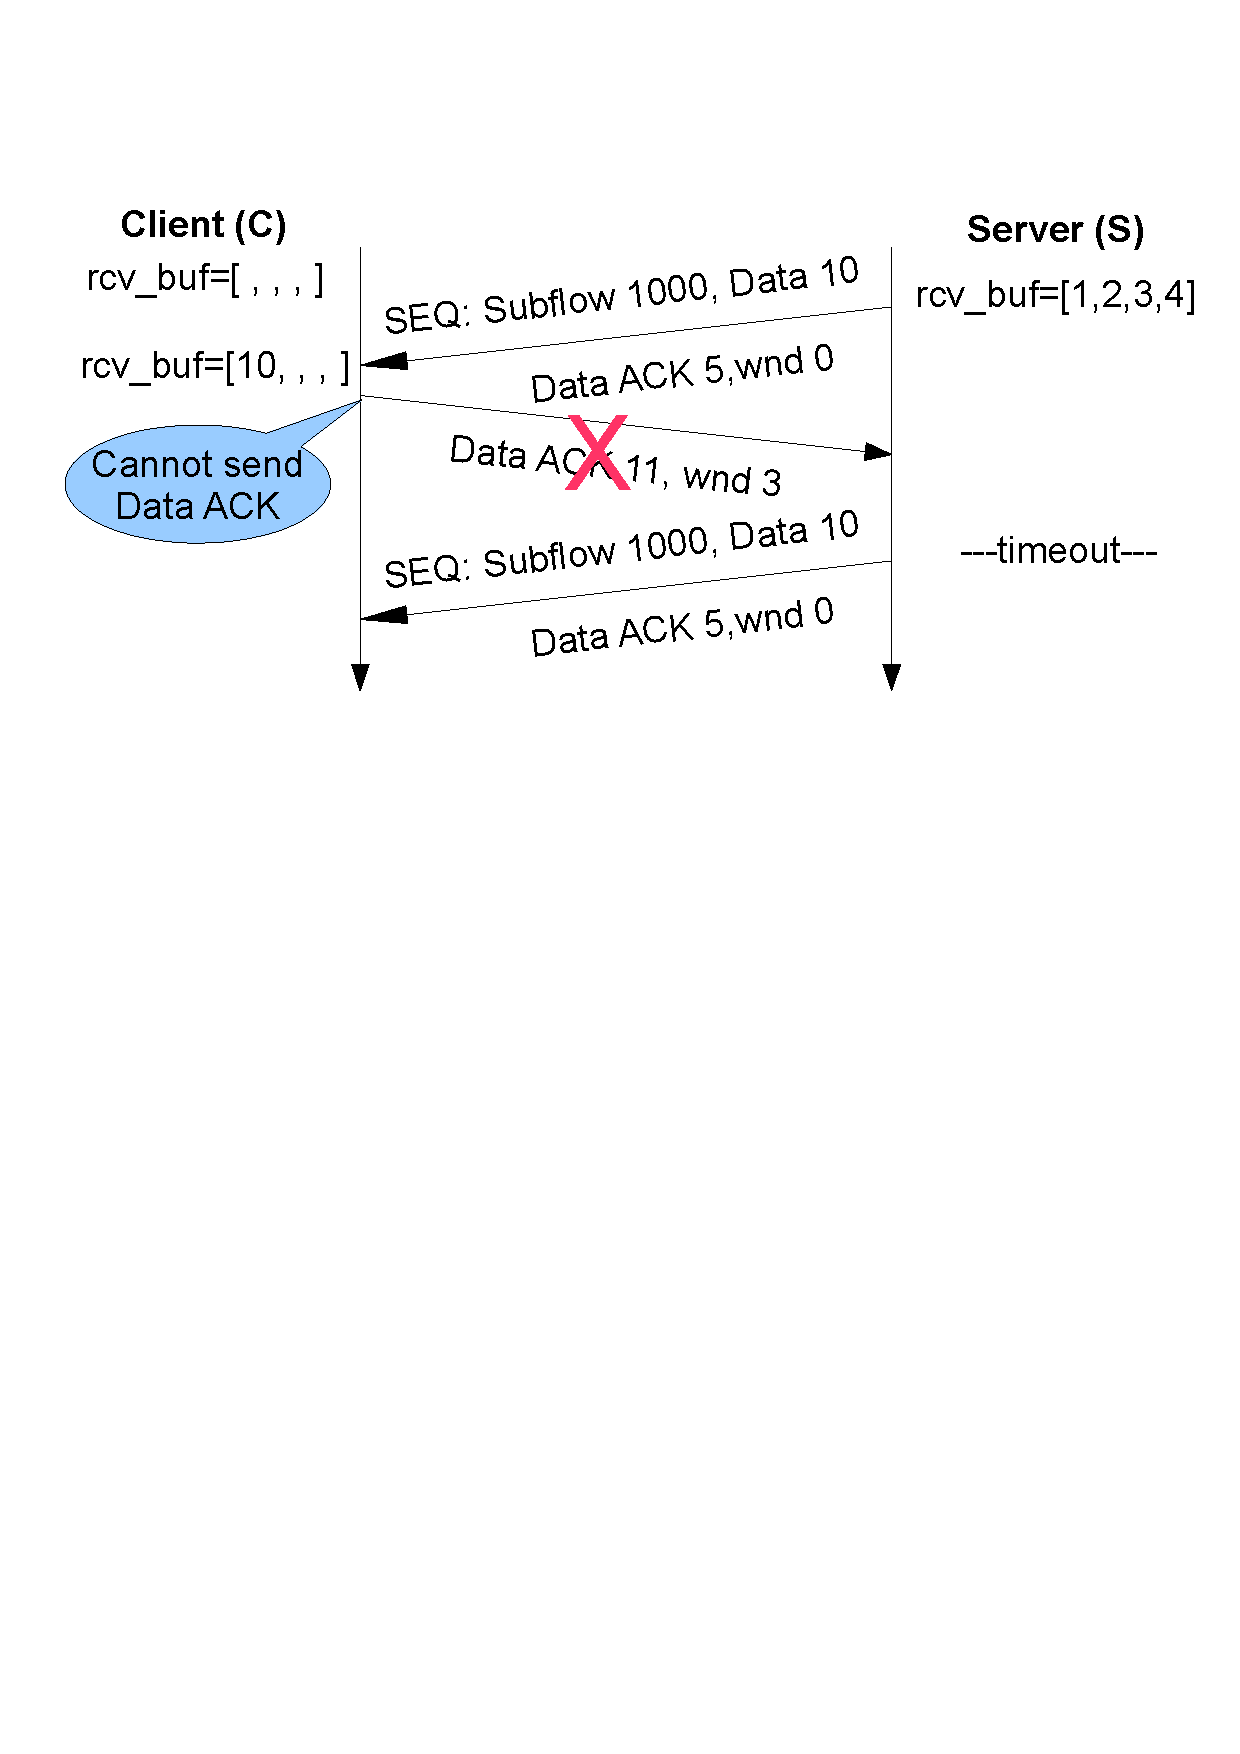
\includegraphics[trim=1cm 17cm 1cm 1cm,clip=true,height=6cm]{figures/dataack_deadlock}
\caption{Flow Control on the path from C to S inadvertently stops the data flow from S to C}
\label{fig:dack_deadlock}
\end{figure}

Flow control presents the most obvious problem for the
chunked payload encoding.  Figure \ref{fig:dack_deadlock} provides an
example. Client C is pipelining requests to server S; meanwhile S's
application is busy sending the large response to the first request so
it isn't yet ready to read the subsequent requests.  At this point,
S's receive buffer fills up.

S sends segment 10, C receives it and wants to send the \texttt{DATA\_ACK}, but
cannot: flow control imposed by S's receive window stops him.
Because no \texttt{DATA\_ACK}s are received from C, S cannot free his send
buffer, so this fills up and blocks the sending application on S.  S's
application will only read when it has finished sending data to C, but
it cannot do so because its send buffer is full.  The send buffer can
only empty when S receives the \texttt{DATA\_ACK} from C, but C cannot send this 
until S's application reads.  This is a classic deadlock cycle.
As no \texttt{DATA\_ACK} is received, S will eventually time out the data it
sent to C and will retransmit it;  after many retransmits the whole connection will time out.

The conclusion is that \texttt{DATA\_ACK}s cannot be safely encoded in the
payload.  The only real alternative is to encode them in TCP options
which (on a pure ACK packet) are not subject to flow control.  

\paragraph{The Data Sequence Mapping.} 
If MPTCP must use options to encode \texttt{DATA\_ACK}s, it is simplest to also
encode the mapping from subflow sequence numbers to data sequence
numbers in a TCP option.  This is the {\em data sequence
mapping} or DSM.

At first glance it seems the {\sc DSM} option simply needs to carry the data
sequence number corresponding to the start of the MPTCP segment.
Unfortunately middleboxes and interfaces that implement TSO or LRO make this far from
simple.  

Middleboxes that re-segment data would cause a problem.
TCP Segmentation Offload (TSO) hardware in the
network interface card (NIC) also re-segments data and is commonly used to improve performance.
The basic idea is that the OS sends large segments and the NIC 
re-segments them to match the receiver's MSS.  What does TSO do 
with TCP options?  A test of 12 NICs supporting
TSO from four different vendors showed that all of them copy a TCP option sent
by the OS on a large segment into all the split segments \cite{raiciu2012hard}.

If MPTCP's DSM option only listed the data sequence number, TSO would
copy the same DSM to more than one segment, breaking the mapping.
Instead the DSM option must say precisely which subflow bytes map to
which data sequence numbers.  But this is further complicated by
middleboxes that modify the initial sequence number of TCP connections
and consequently rewrite all sequence numbers (many firewalls behave like this).
Instead, the {\sc DSM} option must map the offset from the
subflow's initial sequence number to the data sequence number, as the
offset is unaffected by sequence number rewriting.  The option must
also contain the length of the mapping.  This is robust - as long as
the option is received, it does not greatly matter which packet
carries it, so duplicate mappings caused by TSO are not a
problem.

\paragraph{Dealing with Content-Modifying Middleboxes.}
Multipath TCP and content-modifying middleboxes (such as application-level NATs, e.g. for FTP)
have the potential to interact badly.  In particular, due to FTP's ASCII
encoding, re-writing an IP address in the payload can necessitate
changing the length of the payload.  Subsequent sequence and ACK
numbers are then fixed up by the middlebox so they are consistent from
the point of view of the end systems.

Such length changes break the DSM option mapping - subflow bytes can
be mapped to the wrong place in the data stream.  They also
break every other possible mapping mechanism, including chunked
payloads.  There is no easy way to handle such middleboxes.

That is why MPTCP includes an optional checksum in
the DSM mapping to detect such content changes. If an MPTCP host
receives a segment with an invalid DSM checksum, it
rejects the segment and triggers a fallback process:  if any
other subflows exists, MPTCP terminates the subflow on which the
modification occurred;  if no other subflow exists, MPTCP drops back to
regular TCP behavior for the remainder of the connection, allowing the
middlebox to perform rewriting as it wishes. This fallback mechanism
preserves connectivity in the presence of middleboxes.

For efficiency reasons, MPTCP uses the same 16-bit ones complement checksum
used in the TCP header.  This allows the checksum over the payload to
be calculated only once.  The payload checksum is added to a checksum
of an MPTCP pseudo header covering the DSM mapping values and then
inserted into the DSM option.   The same payload checksum is added to the
checksum of the TCP pseudo-header and then used in the TCP checksum field.
MPTCP allows checksums to be disabled for high performance environments such as data-centers where
there is no chance of encountering such an application-level gateway.

The fall-back-to-TCP process, triggered by a checksum failure, can also
be triggered in other circumstances.  For example, if a routing
change moves an MPTCP subflow to a path where a middlebox
removes DSM options, this also triggers the fall-back procedure.


\begin{figure}[t]
\centering
\begin{verbatim}
                      1                   2                   3
  0 1 2 3 4 5 6 7 8 9 0 1 2 3 4 5 6 7 8 9 0 1 2 3 4 5 6 7 8 9 0 1
 +---------------+---------------+-------+----------------------+
 |     Kind      |    Length     |Subtype| (reserved) |F|m|M|a|A|
 +---------------+---------------+-------+----------------------+
 |           Data ACK (4 or 8 octets, depending on flags)       |
 +--------------------------------------------------------------+
 |   Data Sequence Number (4 or 8 octets, depending on flags)   |
 +--------------------------------------------------------------+
 |              Subflow Sequence Number (4 octets)              |
 +-------------------------------+------------------------------+
 |  Data-level Length (2 octets) |      Checksum (2 octets)     |
 +-------------------------------+------------------------------+
\end{verbatim}
\caption{The Data Sequence Signal option in MPTCP that carries the Data Sequence Mapping information,
the Data ACK, the Data FIN and connection-fall-back options. }
\label{fig:mptcp_dss}
\end{figure}

\paragraph{Connection Release.} Multipath TCP must allow a connection to survive
even though its subflows are coming and going. Subflows in MPTCP can be torn down
by means of a four-way handshake as regular TCP flows---this ensures MPTCP
allows middleboxes to clear their state when a subflow is not used anymore.

MPTCP uses an explicit four-way handshake for connection tear-down indicated by a \texttt{DATA\_FIN} option.
The \texttt{DATA\_FIN} is MPTCP's equivalent to TCP's \texttt{FIN}, and it occupies one byte in the data-sequence 
space. A \texttt{DATA\_ACK} will be used to acknowledge the receipt of the \texttt{DATA\_FIN}. MPTCP requires
that the segment(s) carrying a \texttt{DATA\_FIN} must also have the \texttt{FIN} flag set - this ensures
all subflows are also closed when the MPTCP connection is being closed.

For reference, we show the wire format of the option used by MPTCP for data exchange in Figure 
\ref{fig:mptcp_dss}. This option encodes the Data Sequence Mapping, Data ACK, Data FIN and 
the fall-back options. The flags specify which parts of the option are valid, and help reduce option
space usage. 

\subsection{Congestion Control}

One of the most important components in TCP is its congestion controller which 
enables it to adapt its throughput dynamically in response to changing network 
conditions. To perform this functionality, each TCP sender maintains a congestion 
window $w$ which governs the amount of packets that the sender can send without 
waiting for an acknowledgment. The congestion window is updated dynamically 
according to the following rules:

\begin{itemize}
\item On each ACK, increase the window $w$ by $1/w$.
\item Each loss decrease the window $w$ by $w/2$.
\end{itemize}

TCP congestion control ensures fairness:  when multiple connections 
utilize the same congested link each of them will independently converge to the 
same average value of the congestion window.  

What is the equivalent of TCP congestion control for multipath
transport? The obvious question to ask is why not just run regular TCP congestion
control on each subflow?
Consider the scenario in Fig. \ref{fig:1bottleneck}. If multipath
TCP ran regular TCP congestion control on both paths, then the
multipath flow would obtain twice as much throughput as the single
path flow (assuming all RTTs are equal). This is unfair. To solve
this problem, one solution is to try and detect shared bottlenecks
but that is unreliable; a better solution is be less aggressive on
each subflow (i.e. increase window slower) such that in aggregate the MPTCP connection 
is no more aggressive than a single regular TCP connection. 


Before we describe solutions to MPTCP congestion control, let's discuss the three goals that
multipath congestion control must obey \cite{mptcp-cc}:
\begin{enumerate}
\item[\textbf{Fairness}] If several subflows of the same MPTCP connection
share a bottleneck link with other TCP connections, MPTCP should not
get more throughput than TCP. 
\item[\textbf{Deployability}] The performance of all the
Multipath TCP subflows together should be at least that of regular TCP
on any of the paths used by a Multipath TCP connection.  This ensures
that there is an incentive to deploy Multipath TCP. 
\item[\textbf{Efficiency}] A final, most important goal is that Multipath TCP should prefer efficient paths,
which means it should send more of its traffic on paths experiencing
less congestion.
\end{enumerate}

\begin{figure}[t]
\centering
\includegraphics*[width=0.45\columnwidth,bb=167 245 509 380]{figures/1bottleneck}
\caption{A scenario which shows the importance of weighting the aggressiveness of subflows (taken from \cite{mptcp-cc}).}
\label{fig:1bottleneck}
\end{figure}

\begin{figure}[t]
\centering
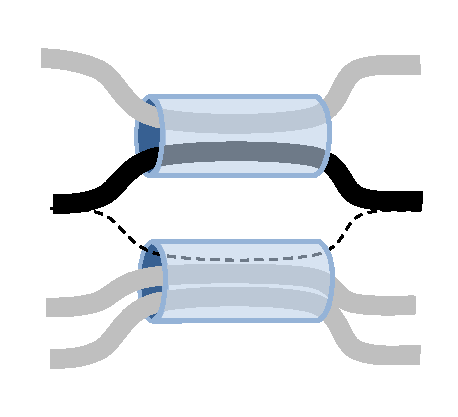
\includegraphics[width=0.5\textwidth]{figures/figure1}
\caption{Two links each with capacity 20~pkts/s. The top link is used by a single TCP connection,
and the bottom link is used by two TCP connections. A Multipath TCP connection uses
both links. Multipath TCP pushes most of its traffic onto less congested top link,
making the two links behave like a resource pool of capacity 40~pkts/s. Capacity is divided equally,
with each flow having throughput 10~pkts/s. (taken from \cite{mptcp-cc})}
\label{fig:mptcp1}
\end{figure}

Intuitively, this last goal ensures wide-area load balancing of traffic: 
when a multipath connection is using two paths loaded unevenly (such as 
Figure \ref{fig:mptcp1}), the multipath transport will prefer the unloaded path
and push most of its traffic there; this will decrease the load on the 
congested link and increase it on the less congested one. 

If a large enough fraction of flows are multipath, congestion will spread 
out evenly across collections of links, creating "resource pools": links 
that act together as if they are a single, larger capacity link shared by 
all flows. This effect is called resource pooling \cite{pooling}.
Resource pooling brings two major benefits, discussed in the paragraphs below.

\paragraph{Increased Fairness.} 
Consider the example shown in Figure \ref{fig:mptcp1}: congestion
balancing ensures that all flows have \textbf{the same throughput}, making
the two links of 20~pkt/s act like a single pooled link with capacity 40~pkt/s 
shared fairly by the four flows. If more MPTCP flows would be added, the two links would still behave as a pool,
sharing capacity fairly among all flows. 
Conversely, if we remove the Multipath TCP flow, the links no longer form a pool, and the throughput allocation
is unfair as the TCP connection using the top path gets twice as much throughput as the TCP connections using the bottom path.


\paragraph{Increased Throughput.}
Consider the somewhat contrived scenario in Fig.\ref{fig:klingon},
and suppose that the three links each have capacity 12Mb/s.
If each flow split its traffic evenly
across its two paths subflow would get 4Mb/s 
hence each flow would get 8Mb/s. But if each flow used only 
the one-hop shortest path, it could get 12Mb/s: this is because
two-hop paths consume double the resources of one-hop paths,
and in a congested network it makes sense to only use the one-hop paths.

\begin{figure}[tb]
\centering
\includegraphics*[width=0.8\columnwidth]{figures/3pipes}
\caption{A scenario to illustrate the importance of choosing the
  less-congested path. (taken from \cite{mptcp-cc})}
\label{fig:klingon}
\end{figure}

In an idle network, however, using all available paths is much better: 
consider the case when only the blue connection is using the links. In this
case this connection would get 24Mb/s throughput; using the one hop path
alone would only provide 12Mb/s.

In summary, the endpoints need to be able to dynamically decide 
which paths to use based on conditions in the network. 
A solution has been devised in the theoretical literature on
congestion control, independently by Kelly and Voice \cite{kelly-voice} and
Han et al. \cite{towsley-cc}.  The core idea is that a multipath flow should
shift all its traffic onto the least-congested path.
In a situation like Fig. \ref{fig:klingon} the
two-hop paths will have higher drop probability than the one-hop
paths, so applying the core idea will yield the efficient
allocation.
Surprisingly it turns out that this can be achieved by doing independent
congestion control at endpoints.

\paragraph{Multipath TCP Congestion Control.}
The theoretical work on multipath congestion control \cite{kelly-voice,towsley-cc} assumes a rate-based
protocol, with exponential increases of the rate. TCP, in contrast, is a packet-based
protocol, sending $w$ packets every round-trip time (i.e. the rate is $w/RTT$); 
a new packet is sent only when an acknowledgment is received, confirming that an existing 
packet has left the network. This property is called ACK-clocking 
and is nice because it has good stability properties:
when congestion occurs round-trip times increase (due to buffering), which
\emph{automatically reduces the effective rate} \cite{Jacobson_congestion:88}.


Converting a theoretical rate-based exponential protocol to a practical 
packet-based protocol fair to TCP turned out to be more difficult than expected. 
There are two problems that appear \cite{mptcp-cc}: 
\begin{itemize}
\item When loss rates are equal on all paths, the theoretical algorithm will
place all of the window on one path or the other, not on both---this effect was termed 
``flappiness'' and it appears because of the discrete (stochastic) nature of packet losses which
are not captured by the differential equations used in theory.
\item The ideal algorithm always prefers paths with lower loss rate, but in practice these may have poor
performance. Consider a mobile phone with WiFi and 3G links: 3G links have very low loss rates and huge round-trip
times, resulting in poor throughput. WiFi is lossy, has shorter round-trip times and typically offers much better throughput.
In this common case, a ``perfect'' controller would place all traffic on the 3G path, violating the second goal (deployability).
\end{itemize}

The pragmatic choice is to sacrifice some load-balancing ability to ensure greater stability and
to offer incentives for deployment. This is what Multipath TCP congestion control does.

Multipath TCP congestion control is a series of simple changes to the standard TCP congestion control mechanism. Each subflow 
has its own congestion window, that is halved when packets are lost, as in standard TCP \cite{mptcp-cc}.

Congestion balancing is implemented in the increase phase of 
congestion control: here Multipath TCP will allow less congested subflows 
to increase proportionally more than congested ones. Finally, the total 
increase of Multipath TCP across all of its subflows is dynamically chosen 
in such a way that it achieves the first and second goals above. 

The exact algorithm is described below and it satisfies the goals we've discussed:
\begin{itemize}
\item Upon ACK on subflow $r$, increase the window $w_r$ by
$\min(a/w_{total}),1/w_r)$.
\item Upon loss on subflow $r$, decrease the window $w_r$ by $w_r/2$.
\end{itemize}
Here
\begin{equation}
\label{eq:a}
a = w_{total} \frac{\max_r w_r/RTT_r^2}{(\sum_r
  w_r/RTT_r)^2},
\end{equation}
$w_r$ is the current window size on subflow $r$ and $w_{total}$ is the
sum of windows across all subflows. 

The algorithm biases the increase towards uncongested paths: these will receive
more ACKs and will increase accordingly. However, MPTCP does keep some traffic
even on the highly congested paths; this ensures stability and allows it
to quickly detect when path conditions improve.

$a$ is a term that is computed dynamically upon each packet drop. Its purpose 
is to make sure that MPTCP gets at least as much throughput as TCP on the best path.
To achieve this goal, $a$ is computed by estimating how much TCP would get on each MPTCP path
(this is easy, as round-trip time and loss-rates estimates are known) and ensuring that MPTCP
in stable state gets at least that much. A detailed discussion on the design of the MPTCP congestion
control algorithm is provided in \cite{mptcp-cc}.

For example, in the three-path example above, the flow will put
45\% of its weight on each of the less congested path and 10\% on the
more congested path. This is intermediate between regular TCP
(33\% on each path) and a perfect load balancing algorithm (0\% on the more congested path)
that is impossible to implement in practice.

The window increase is capped at $1/w_r$, which ensures that
the multipath flow can take no more capacity on either path than a
single-path TCP flow would.

In setting the $a$ parameter, Multipath TCP congestion control uses subflow delays to compute the target rate.
Using delay for congestion control is not a novel idea: TCP Vegas \cite{vegas}, for instance, performs
congestion control only by tracking RTT values. Vegas treats increasing RTTs as a sign of congestion, instead
of relying on packet losses as regular TCP does. That is why Vegas loses out to regular TCP at shared bottlenecks,
and is probably the reason for its lack of adoption. MPTCP does not treat delay as congestion: it just uses it
to figure out the effective rate of a TCP connection on a given path. This allows MPTCP to compete fairly with TCP.

\paragraph{Alternative Congestion Controllers for Multipath TCP.} The standardized Multipath
TCP congestion control algorithm chooses a trade-off between load balancing, stability and
the ability to quickly detect available capacity. The biggest contribution of this
work is the clearly defined goals for what multipath congestion control should do,
and an instantiation that achieves (most of) the stated goals in practice.

This research area is relatively new, and it is likely that more work will lead to better 
algorithms---if not generally applicable, then at least tailored to some practical use-cases.
A new and interesting congestion controller called Opportunistic Linked Increases Algorithm (OLIA) 
has already been proposed \cite{olia} that offers better load balancing with seemingly few drawbacks.

We expect this area to be very active in the near future; of particular interest are designing multipath
versions of high-speed congestion control variants deployed in practice, such as Cubic or Compound TCP. 



\subsection{Implementation and performance}

We now briefly cover two of the most compelling use cases for
Multipath TCP by showing a few evaluation results. We focus on mobile
devices and datacenters but note that Multipath TCP can also help in
other scenarios.  For example, multi-homed web-servers can perform
fine-grained load-balancing across their uplinks, while dual-stack
hosts can use both IPv4 and IPv6 within a single Multipath TCP
connection.

The full Multipath TCP protocol has been implemented in the Linux
kernel; its congestion controller has also been implemented in the ns2
and htsim network simulators. The results presented in here are from
the Linux kernel implementation \cite{raiciu2012hard}. 

\begin{figure}[t]
\centering
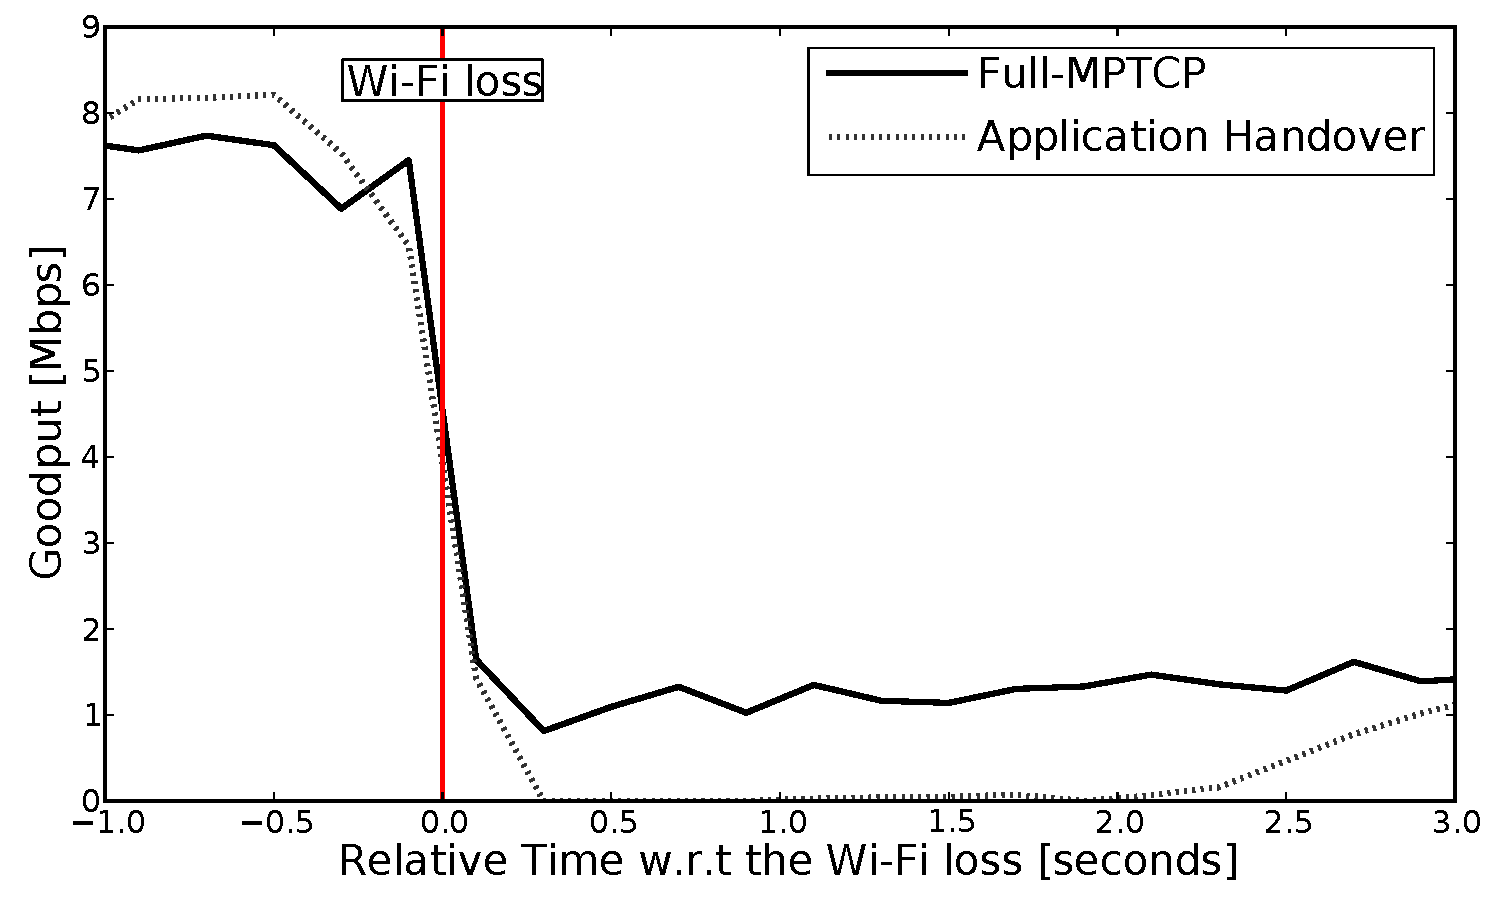
\includegraphics[width=0.5\textwidth]{figures/figure2}
\caption{(Mobility) A mobile device is using both its WiFi and 3G interfaces, and then the WiFi
interface fails. We plot the instantaneous throughputs of Multipath TCP and application-layer
handover. (taken from \cite{Paasch_Mobile:2012})} 
\label{fig:mptcp2}
\end{figure}

The mobile measurements focus on a typical mode of operation where the device is 
connected to WiFi, the connection goes down and the phone switches to using 3G. 
The setup uses a Linux laptop connected to a WiFi and a 3G network, downloading a 
file using HTTP. 

3G to Wifi handover is implemented in today's phones by changing the application to monitor
the network interfaces. When the app detects the loss of the interface, it creates a new TCP connection 
to the server and the connection can resume. This solution, while simple, is not applicable to all applications
because some of the bytes succesfully delivered by the old connection may be resent by the new one.

Applications that rely on HTTP GET requests (with no side effects) are, however, easy to change. The 
HTTP range header allows a client to resume the download of a file from a specified offset. This is the de-facto
standard for today's apps.  

Figure \ref{fig:mptcp2} compares application layer-handover (with HTTP-range) against Multipath TCP.
The figure shows a 
smooth handover with Multipath TCP, as data keeps flowing despite the interface 
change. With application-layer handover there is a downtime of 4 seconds where the transfer 
stops-this is because it takes time for the application to detect the interface down 
event, and it takes time for 3G to ramp up. 

Multipath TCP enables unmodified mobile applications to survive interface changes with
little disruption. Selected apps can be modified today to support handover, but their performance
is worse than with MPTCP. A more detailed discussion of the utilization of
Multipath TCP in WiFi/3G environments may be found in \cite{Paasch_Mobile:2012}.

\begin{figure}[t]
\centering
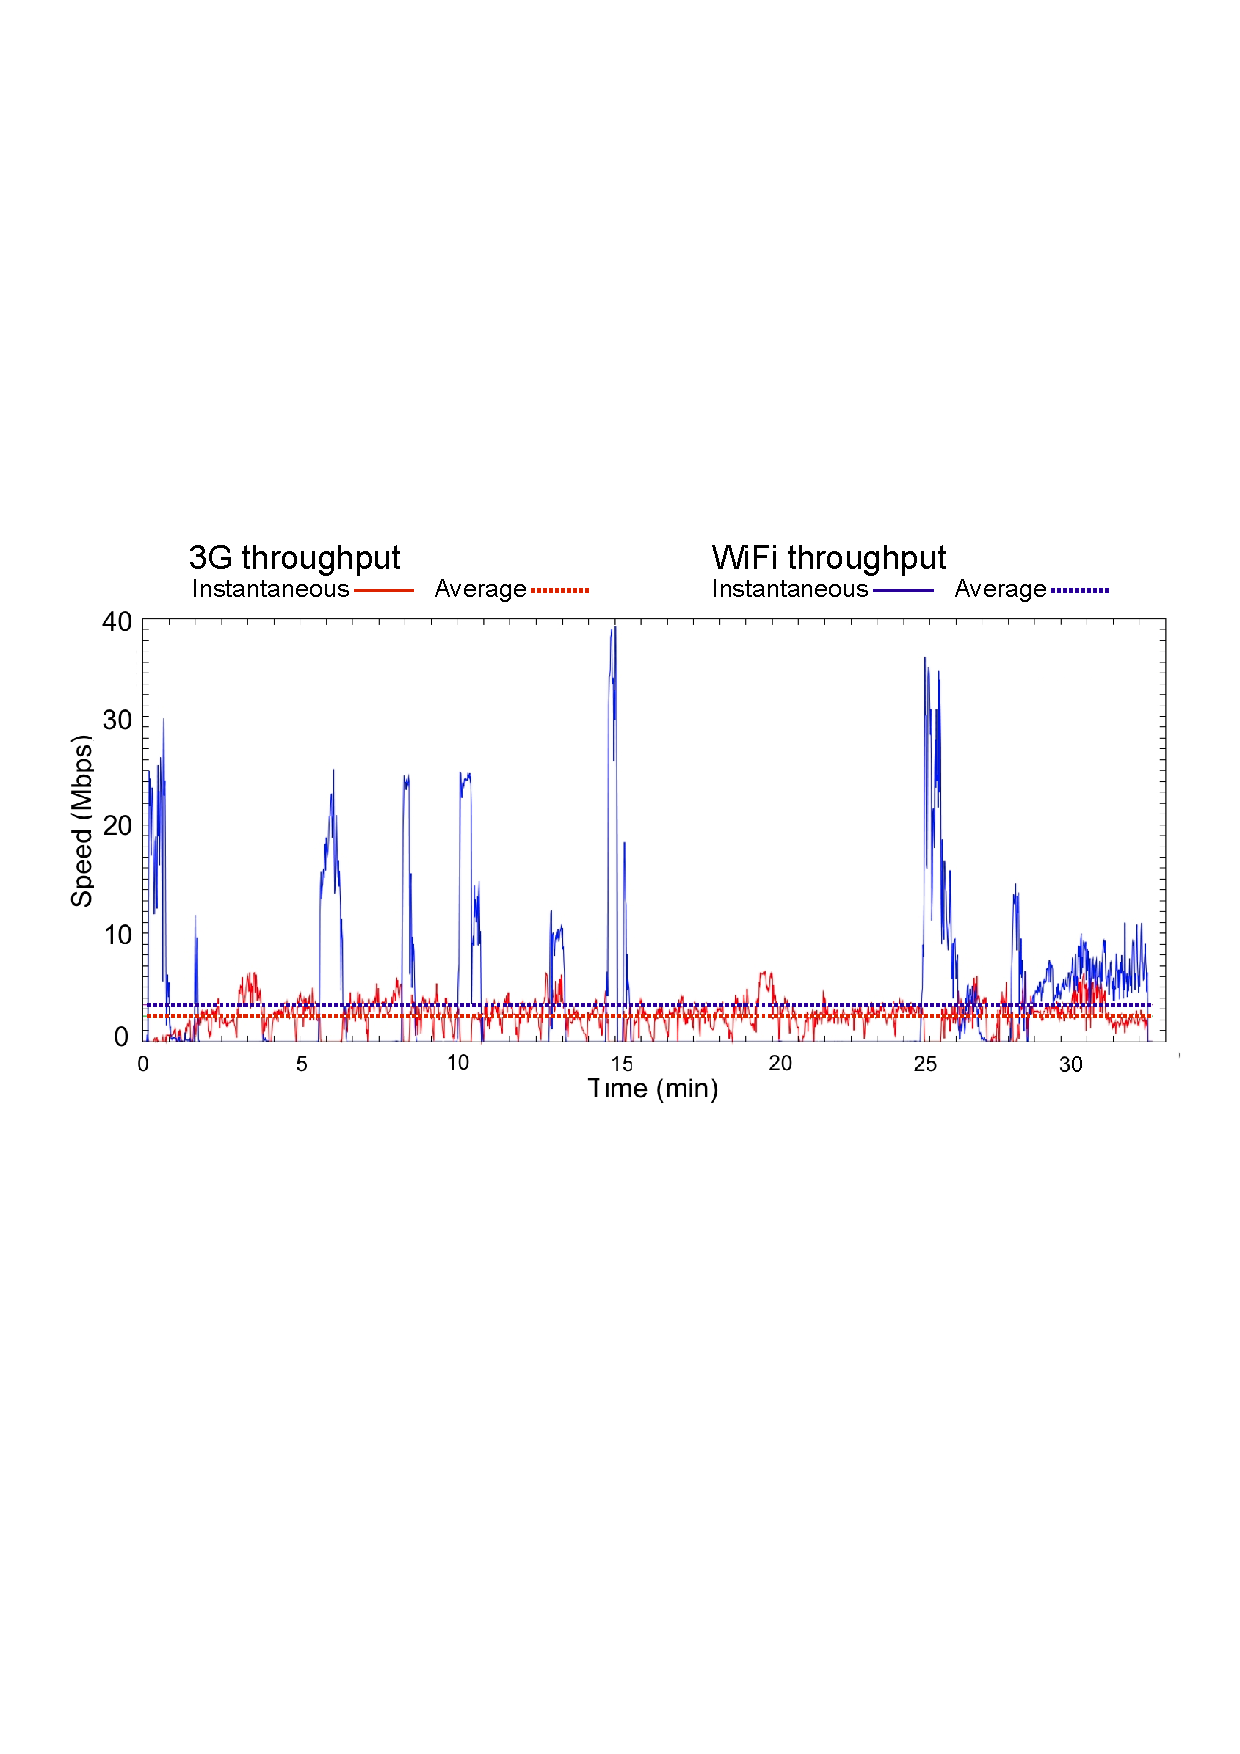
\includegraphics[width=\textwidth,trim=0 11cm 0 9cm,clip=true]{figures/throughput-subway}
\caption{(3G to WiFi Handover) A Linux distribution is downloaded by a mobile user while on the Bucharest subway. 3G coverage is ubiquitous. WiFi is available only in stations.}
\label{fig:throughput-subway}
\end{figure}

We also present a real mobility trace in Figure \ref{fig:throughput-subway}, where a mobile user downloads a Linux distro on his laptop
while travelling on the Bucharest underground. The laptop uses a 3G dongle to connect to the cellular network and its WiFi NIC to connect 
to access points available in stations. 

The figure shows the download speeds of the two interfaces during a 30 minute underground ride. 3G throughput is stable: the average is 
2.3Mbps (shown with a dotted line on the graph), and the instantaneous throughput varies inversely proportional with the distance 
to the 3G cell. WiFi throughput is much more bursty: in some stations the throughput soars to 40Mbps, while in others it is zero, as 
the laptop doesn't manage to associate and obtain an IP address quickly enough. The average WiFi throughput (3.3Mbps) is higher 
than the average 3G throughput.

While MPTCP uses both interfaces in this experiment, using just WiFi when it is available may be preferable as it reduces 3G data bills
and reduces the load of the cellular network. This is easy to implement with MPTCP, as it supports a simple  prioritization mechanism 
that allows the client to inform the server to send data via preferred subflow(s) \footnote{MPTCP sends an MP\_PRIO option to 
inform the remote end about changes in priority for the subflows.}. 


\begin{figure}[t]
\centering
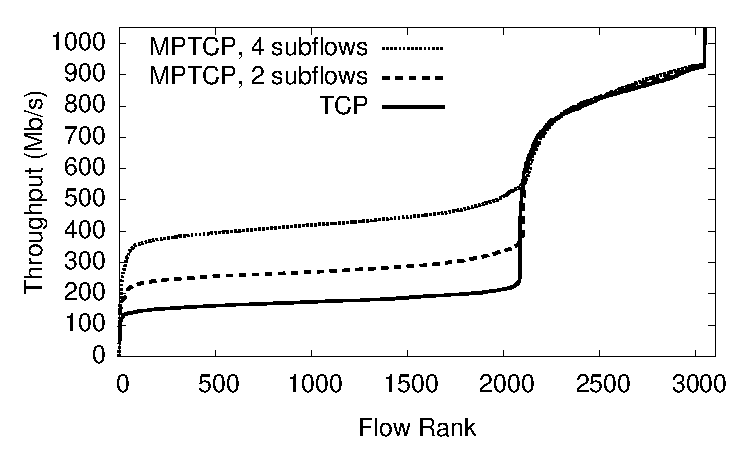
\includegraphics[width=0.5\textwidth]{figures/figure3}
\caption{(Datacenter load-balancing) This graph compares standard TCP with MPTCP 
with two and four flows, when tested on an EC2 testbed with 40 instances. Each host 
uses iperf sequentially to all other hosts. We plot the performance of all flows (Y axis)
in increasing order of their throughputs (X axis). (taken from \cite{raiciu2011improving})}
\label{fig:mptcp3}
\end{figure}

\paragraph{Datacenters.} We also show results from running Multipath TCP in a different scenario: the EC2 datacenter.
Like most datacenters today, EC2 uses a redundant network topology where many paths are 
available between any pair of endpoints, and where connections are placed randomly 
onto available paths. In EC2, 40 machines (or instances) ran the 
Multipath TCP kernel. A simple experiment was run where every machine measured
the throughput sequentially to every other machine using first TCP, then Multipath 
TCP with two and with four subflows. Figure \ref{fig:mptcp3} shows the sorted throughputs measured over 
12 hours. The results show that Multipath TCP brings significant improvements compared 
to TCP in this scenario. Because the EC2 network is essentially a black-box , it is 
difficult to pinpoint the root cause for the improvements; however, a
detailed analysis of the cases where Multipath TCP can help and why in is presented in 
\cite{raiciu2011improving}.

\subsection{Impact of Multipath TCP}

MPTCP is deployable today, as it was designed and shown to work over existing networks and unmodified applications.
Whether MPTCP will be adopted or not is unclear at this point; only time will tell.
If MPTCP is adopted, however, it will likely affect the development of both the network and the applications running 
on top of it. Here we briefly speculate on what the impact might be. 
Multipath TCP embeds two key mechanisms: load balancing to avoid congested paths, and the ability 
to use different IP addresses in the same connection. Having these mechanisms implemented at the end-hosts
means other layers (e.g. the network) may become simpler, and more efficient.

For instance, MPTCP seamlessly uses available bandwidth even if it is short-lived (e.g. WiFi in underground stations), 
and provides robustness when a subset of paths fail by quickly resending data on working paths. This could take
some of the load imposed on BGP, that today must quickly reconverge in the case of a failure. With MPTCP at the endpoints
failures would be ``masked'' automatically, allowing BGP to react to failures slowly which will ensure there are no 
oscillations. However, one must ensure that the paths used by the end-systems are disjoint and that the failure
does not affect all of them.

Another example is layer 2 mobility, implemented in both WiFi and cellular networks, that aims to do a fast handover from 
one access point to the next, or from one cell to the next. With MPTCP as a transport protocol, a WiFi client could connect
simultaneously to two access points or cells (provided the L2 protocol allows it), and load balance traffic on the best 
link. MPTCP could replace fast handovers with slow handovers that are more robust. Of course, some changes may be needed 
at layer 2 to support such load balancing.

Network topologies may be designed differently if MPTCP is the transport protocol. An example is GRIN \cite{grin}, a work that
proposes to change existing datacenter networks by randomly interconnecting servers in the same rack directly, using their free 
NIC ports. This allows a server to opportunistically send traffic at speeds larger than its access link by having its idle neighbor 
relay some traffic on its behalf. With a minor topology change and MPTCP, GRIN manages to better utilize the datacenter network core.

The mechanisms that allow MPTCP to use different IPs in the same transport connection (i.e. the connection identifier) 
also allow connections to be migrated across physical machines with different IP addresses. One direct application is seamless virtual
machine migration: an MPTCP-enabled guest virtual machine can just resume its connections after it is migrated.

On the application side many optimizations are possible. Applications like video
and audio streaming only need a certain bitrate to ensure user satisfaction - they rarely fully utilize the wireless capacity.
Our mobility graph in the previous section shows that, in principle, WiFi has enough capacity to support these apps, even if it is 
only available in stations. A simple optimization would be to download as much of the video as possible while on WiFi, and only
use 3G when the playout buffer falls below a certain threshold. This would ensure a smooth viewing experience while pushing as 
much traffic as possible over WiFi. 

The examples shown in this section are only meant to be illustrative, and their potential impact or even feasibility 
is not clear at this point. Further, the list is not meant to be exhaustive. 
We have only provided it to show that Multipath TCP benefits go beyond than
increasing throughput, and could shape both the lower and the upper layers of the protocol stack in the future.


\section{Minion}\label{section:minion}
%%%%%%%%%%%%%

\def\utcp{$u$TCP\xspace}
\def\utls{$u$TLS\xspace}
\def\ucobs{$u$COBS\xspace}

As the Internet has grown and evolved
over the past few decades,
congestion control algorithms and extensions such as MPTCP
continue to reflect an evolving TCP.
However,
a proliferation of middleboxes
such as 
Network Address Translators (NATs), 
Firewalls,
and 
Performance Enhancing Proxies (PEPs),
has arguably stretched the waist of the Internet hourglass
upwards from IP
to include
TCP and UDP~\cite{rosenberg08udp, ford08breaking, popa10http},
making it increasingly difficult
to deploy new transports
and to
use anything but TCP and UDP 
on the Internet.

TCP~\cite{rfc793} was originally designed to offer applications
a convenient, high-level communication abstraction
with semantics emulating Unix file I/O or pipes:
a reliable, ordered bytestream,
through an end-to-end channel (or connection).
As the Internet has evolved, however,
applications needed better abstractions
from the transport.
We start this section by examining
how TCP's role in the network has evolved
from a communication {\em abstraction} to a communication {\em substrate},
why its in-order delivery model makes TCP a poor substrate,
why other OS-level transports have failed to replace TCP in this role,
and why UDP is inadequate as the only alternative substrate to TCP.

\subsection{Rise of Application-Level Transports}

The transport layer's traditional role in a network stack
is to build high-level communication abstractions
convenient to applications,
atop the network layer's basic packet delivery service.
TCP's reliable, stream-oriented design~\cite{rfc793}
exemplified this principle,
by offering an inter-host communication abstraction
modeled on Unix pipes,
which were the standard {\em intra-host} communication abstraction
at the time of TCP's design.
The Unix tradition of
implementing TCP in the OS kernel
offered further convenience,
allowing much application code to ignore the difference between
an open disk file, an intra-host pipe, or an inter-host TCP socket.

\begin{figure}[tbp]
\centering
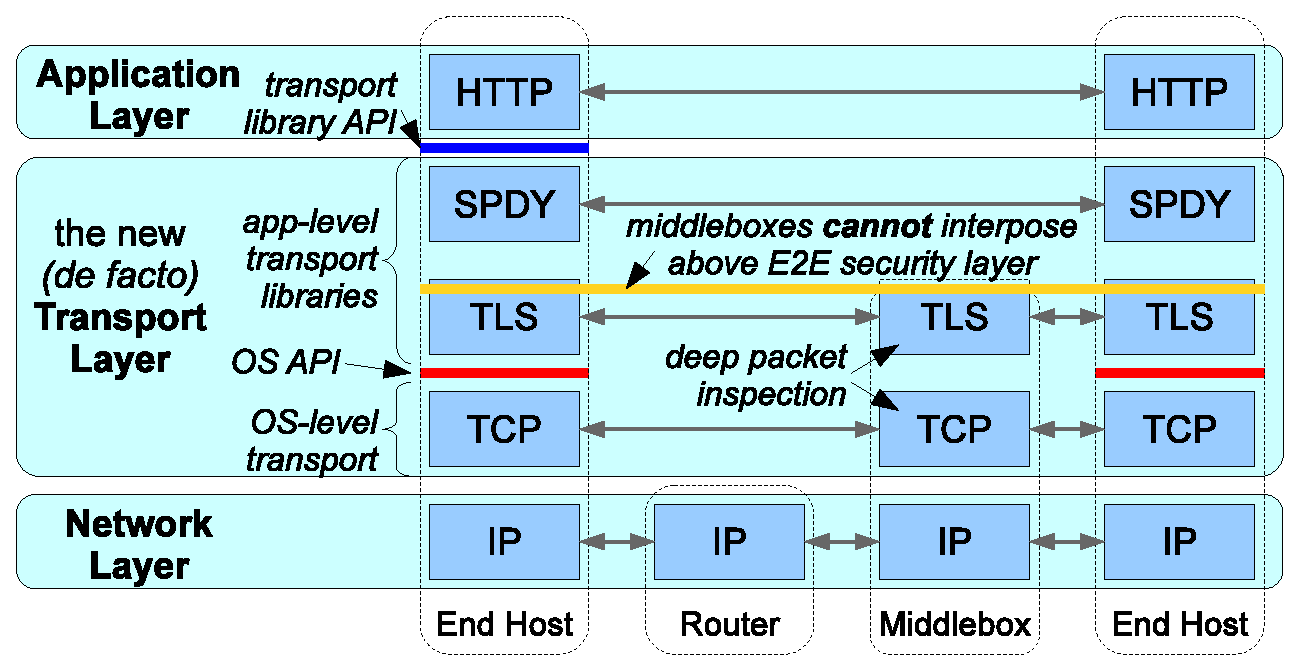
\includegraphics[width=0.8\textwidth]{figures/layers.eps}
\caption{Today's ``{\em de facto} transport layer''
	is effectively split between OS and application code. (taken from
    \cite{nowlan12fitting})}
\label{f:layers}
\end{figure}

Instead of building directly atop
traditional OS-level transports such as TCP or UDP, however,
today's applications
frequently introduce additional transport-like
protocol layers at user-level,
typically implemented via application-linked libraries.
Examples include the ubiquitous SSL/TLS~\cite{rfc5246},
media transports such as RTP~\cite{rfc3550},
and experimental multi-streaming transports such as
SST~\cite{ford07structured}, SPDY~\cite{spdy},
and \O{}MQ~\cite{zeromq}.
Applications increasingly use HTTP or HTTPS over TCP
as a substrate~\cite{popa10http};
this is also illustrated by 
the W3C's WebSocket interface~\cite{websocket},
which offers general bidirectional communication
between browser-based applications and Web servers atop HTTP and HTTPS.

In this increasingly common design pattern,
the ``transport layer'' as a whole has in effect become
a stack of protocols straddling the OS-application boundary.
Figure~\ref{f:layers} illustrates one example stack,
representing Google's experimental Chrome browser,
which inserts SPDY for multi-streaming and TLS for security
at application level,
atop the OS-level TCP.

One can debate whether a given application-level protocol
fits some definition of ``transport'' functionality.
The important point, however,
is that {\em today's applications no longer need, or expect,
the underlying OS to provide ``convenient'' communication abstractions:
an application simply links in libraries, frameworks,
or middleware offering the abstractions it desires.}
What today's applications
need from the OS is not convenience,
but {\em an efficient substrate}
atop which application-level libraries
can build the desired abstractions.

\subsection{TCP's Latency Tax}

While TCP has proven to be a popular
substrate for application-level transports,
using TCP in this role
converts its delivery model from a blessing into a curse.
Application-level transports are just as capable as the kernel
of sequencing and reassembling packets into
a logical data unit or ``frame''~\cite{clark90architectural}.
By delaying any segment's delivery to the application
until all prior segments are received and delivered, however,
TCP imposes a ``latency tax'' on all segments
arriving within one round-trip time (RTT) after any single lost segment.

This latency tax is a fundamental byproduct
of TCP's in-order delivery model,
and is irreducible,
in that an application-level transport
cannot ``claw back''
the time a potentially useful segment
has wasted in TCP's buffers.
The best the application can do is
simply to {\em expect} higher latencies to be common.
A conferencing application can use a longer jitter buffer,
for example,
at the cost of increasing user-perceptible lag.
Network hardware advances are unlikely to address this issue, 
since TCP's latency tax depends on RTT,
which is lower-bounded by the speed of light
for long-distance communications.

\subsection{Alternative OS-level Transports}
\label{sec:motiv-alts}

All standardized OS-level transports since TCP, including
	UDP~\cite{rfc768}, RDP~\cite{rfc908},
	DCCP~\cite{rfc4340}, and SCTP~\cite{rfc4960},
support out-of-order delivery.
The Internet's evolution has created strong barriers
against the widespread deployment of new transports
other than the original TCP and UDP, however.
These barriers are detailed elsewhere~\cite{
	rosenberg08udp,ford08breaking,popa10http},
but we summarize two key issues here.

First, 
adding or enhancing a ``native'' transport built atop IP
involves modifying popular OSes,
effectively increasing the bar for widespread deployment
and making it 
more difficult to evolve transport functionality
below the red line representing the OS API
in Figure~\ref{f:layers}.
Second, the Internet's original ``dumb network'' design,
in which routers that ``see'' only up to the IP layer,
has evolved into a ``smart network''
in which pervasive middleboxes
perform deep packet inspection and interposition
in transport and higher layers.
Firewalls tend to block ``anything unfamiliar'' for security reasons,
and Network Address Translators (NATs)
rewrite the port number in the  transport header,
making both incapable of allowing traffic from a new transport
without explicit support for that transport.
Any packet content
not protected by end-to-end security such as TLS---%
the yellow line in Figure~\ref{f:layers}---%
has become ``fair game''
for middleboxes to inspect and interpose on~\cite{
	reis08detecting},
making it more difficult to evolve transport functionality
anywhere below that line.


\subsection{Why Not UDP?}

As the only widely-supported transport
with out-of-order delivery,
UDP offers a natural
substrate for application-level transports.
Even applications otherwise well-suited to UDP's delivery model
often favor TCP as a substrate, however.

A recent study found over 70\% of streaming media using TCP~\cite{
	guo06delving},
and even latency-sensitive conferencing applications
such as Skype
often use TCP~\cite{baset06analysis}.
Firewalls can monitor the TCP state machine
to help thwart network attacks~\cite{handley01network},
but determining an application session's state atop UDP
requires application-specific analysis~\cite{northcutt05inside},
creating an incentive for firewalls to block UDP in general.

In general,
network middleboxes support UDP widely but not {\em universally}.
For this reason,
latency-sensitive applications
seeking maximal connectivity ``in the wild''
often fall back to TCP when UDP connectivity fails.
Skype~\cite{baset06analysis}
and Microsoft's Direct\-Access VPN~\cite{davies09directaccess},
for example,
support UDP but can masquerade
as HTTP or HTTPS streams atop TCP when required for connectivity.

TCP can offer performance advantages over UDP as well.
For applications requiring congestion control,
an OS-level implementation in TCP
may be more timing-accurate
than an application-level implementation in a UDP-based protocol,
because the OS kernel
can avoid the timing artifacts of 
system calls and process scheduling~\cite{zec02estimating}.
Hardware TCP offload engines
can optimize common-case efficiency
in end hosts~\cite{mogul03tcp},
and performance enhancing proxies
can optimize TCP throughput across diverse networks~\cite{
	rfc3234,cisco-rbscp}.
Since middleboxes can track TCP's state machine,
they impose much longer idle timeouts on open TCP connections---%
nominally two hours~\cite{rfc5382}---%
whereas UDP-based applications must send keepalives
every two minutes to keep an idle connection open~\cite{rfc4787},
draining power on mobile devices.

\subsection{Breaking Out Of the Transport Logjam}
Applications and application developers care most about 
services that the networking infrastructure offers to them
and not how packets look on the wire;
that is, they care about 
new transport {\em services}, not new transport {\em protocols}.
On the other hand,
middleboxes care most about how packets look on the wire,
and generally do not care about what services are offered to the applications;
that is, changing the transport protocol's bits on the wire
will require changing middleboxes to respond to these changes as well.

For application developers,
TCP versus UDP represents an ``all-or-nothing'' choice
on the spectrum of services applications need.
Applications desiring some but not all of TCP's services,
such as congestion control but unordered delivery,
must reimplement and tune all other services atop UDP
or suffer TCP's performance penalties.

Without dismissing UDP's usefulness 
as a truly ``least-common-denominator'' substrate,
we believe the factors above
suggest that TCP will also remain a popular substrate---%
even for latency-sensitive applications
that can benefit from out-of-order delivery---%
and that a deployable, backward-compatible workaround
to TCP's latency tax
can significantly benefit such applications.

Recognizing that the development of application-level transports
and the use of TCP as a substrate under them
is likely to continue and expand,
we now describe {\em Minion},
an architecture for efficient but backward-compatible
unordered delivery over extant transports, including TCP.
Minion consists of
{\em \utcp},
a small OS extension
adding basic unordered delivery primitives to TCP,
and two application-level protocols
implementing datagram-oriented delivery services
that function on either \utcp or unmodified TCP stacks.

While building a new transport on UDP 
or using alternative OS-level transports where available
are both perfectly reasonable design approaches,
Minion offers a uniform interface for applications to use
along with an alternative option
where the ubiquitous TCP protocol is adequate, but the sockets API is not;
where a new transport service
can be offered using TCP's bits on the wire.

\subsection{Minion Architecture Overview}

Minion is an architecture and protocol suite
designed to provide efficient unordered delivery built atop
existing transports.
Minion itself offers no high-level abstractions:
its goal is to serve
applications and higher application-level transports,
by acting as a ``packhorse''
carrying raw datagrams as reliably and efficiently as possible
across today's diverse and change-averse Internet.

\begin{figure}[tbp]
\centering
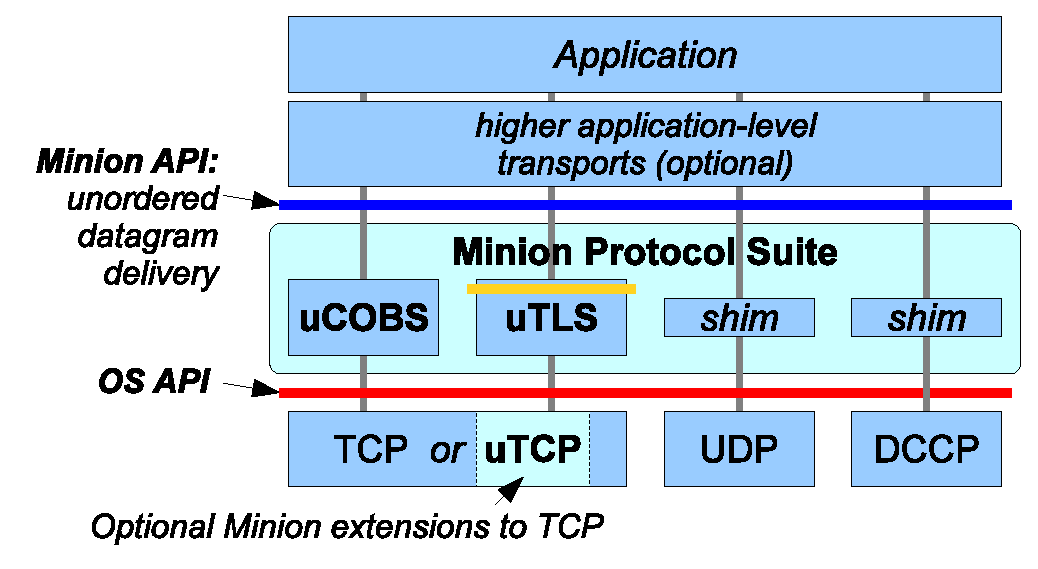
\includegraphics[width=0.6\textwidth]{figures/minionarch.eps}
\caption{Minion architecture (taken from~\cite{nowlan12fitting})}
\label{f:minionarch}
\end{figure}

Figure~\ref{f:minionarch} illustrates Minion's architecture.
Applications and higher application-level transports
link in and use Minion in the same way as they already use
existing application-level transports
such as DTLS~\cite{rfc4347},
the datagram-oriented analog of SSL/TLS~\cite{rfc5246}.
In contrast with DTLS's goal of layering security
atop datagram transports such as UDP or DCCP,
Minion's goal is to offer efficient datagram delivery
atop {\em any} available OS-level substrate, including TCP.

Minion consists of
several application-level transport protocols,
%in the spirit of Section~\ref{sec:motiv},
together with a set of optional enhancements
to end hosts' OS-level TCP implementations.

Minion's enhanced OS-level TCP stack,
called {\em \utcp} (``unordered TCP''),
includes sender- and receiver-side
API features supporting unordered delivery and prioritization,
as detailed later in this section.
These enhancements affect only the OS API
through which application-level transports such as Minion
interact with the TCP stack,
and make {\em no} changes to TCP's wire protocol.

Minion's application-level protocol suite currently consists
of the following main components:
\begin{itemize}
\item	{\bf \ucobs} is a protocol
	that implements a minimal unordered datagram delivery service
	atop either unmodified TCP or \utcp,
	using 
    {\em Consistent-Overhead Byte Stuffing}, or
    COBS encoding~\cite{cheshire97consistent}
	to facilitate out-of-order datagram delimiting
	and prioritized delivery,
	as described later in Section~\ref{sec:dgrams_utcp}.
\item	{\bf \utls} is a modification of
	the traditionally stream-oriented TLS~\cite{rfc5246},
	offering a secure, unordered datagram delivery service
	atop TCP or \utcp.
	The wire-encoding of \utls streams
	is designed to be indistinguishable in the network
	from conventional, encrypted TLS-over-TCP streams (e.g., HTTPS),
	offering a maximally conservative design point
	that makes no network-visible changes
	``below the yellow line''
	in Figure~\ref{f:minionarch}.
	Section~\ref{sec:dgrams_utcp} describes \utls.
\item	Minion adds shim layers
	atop OS-level datagram transports, such as UDP and DCCP,
	to offer applications a consistent API
	for unordered delivery across multiple OS-level transports.
	Since these shims are merely wrappers
	for OS transports already offering unordered delivery,
	this paper does not discuss them in detail.
\end{itemize}

Minion currently leaves to the application
the decision of {\em which} protocol to use for a given connection:
e.g., \ucobs or \utls atop TCP/\utcp,
or OS-level UDP or DCCP via Minion's shims.
Other ongoing work explores {\em negotiation protocols}
to explore the protocol configuration space dynamically,
optimizing protocol selection and configuration
for the application's needs and the network's 
constraints~\cite{ford09efficient}.
Many applications already incorporate simple negotiation schemes,
however---%
e.g., attempting a UDP connection first
and falling back to TCP if that fails---%
and adapting these mechanisms
to engage Minion's protocols according to
application-defined preferences and decision criteria
should be straightforward.

\subsection{Compatibility and Deployability}

Minion addresses the key barriers to transport evolution,
outlined in Section~\ref{sec:motiv-alts},
by creating a backward-compatible, incrementally deployable substrate
for new application-layer transports desiring unordered delivery.
Minion's deployability rests on the fact that it can,
when necessary,
avoid relying on changes either
``below the red line'' in the end hosts
(the OS API in Figure~\ref{f:minionarch}),
or
``below the yellow line'' in the network
(the end-to-end security layer in Figure~\ref{f:minionarch}).

While Minion's \ucobs and \utls protocols
offer maximum performance benefits from out-of-order delivery
when both endpoints include OS support for Minion's \utcp enhancements,
\ucobs and \utls still function and interoperate correctly
even if neither endpoint supports \utcp,
and the application need not know or care
whether the underlying OS supports \utcp.
If only one endpoint OS supports \utcp,
Minion still offers incremental performance benefits,
since \utcp's sender-side and receiver-side enhancements are independent.
A \ucobs or \utls connection atop a mixed TCP/\linebreak[0]\utcp endpoint-pair
benefits from \utcp's sender-side enhancements
for datagrams sent by the \utcp endpoint,
and the connection benefits from \utcp's receiver-side enhancements
for datagrams arriving at the \utcp host.

Addressing the challenge of network-compatibility
with middleboxes that filter new OS-level transports
and sometimes UDP,
Minion offers application-level transports
a continuum of substrates
representing different tradeoffs
between suitability to the application's needs
and compatibility with the network.

An application can use unordered OS-level transports
such as UDP, DCCP~\cite{rfc4340}, or SCTP~\cite{rfc4960},
for paths on which they operate,
but Minion offers an unordered delivery alternative
wire-compatible not only with TCP,
but with the ubiquitous TLS-over-TCP streams
on which HTTPS (and hence Web security and E-commerce) are based,
likely to operate in almost any network environment
purporting to offer ``Internet access.''

\subsection{Minion's Unordered Delivery using TCP and TLS}
We now briefly discuss Minion's true unordered delivery
over bytestream protocols;
we describe how Minion provides true unordered datagram
delivery without modifying the TCP and TLS wire-formats.

Minion enhances the OS's TCP stack
with API enhancements supporting unordered delivery
in both TCP's send and receive paths,
enabling applications to reduce transmission latency
at both the sender- and receiver-side end hosts
when both endpoints support \utcp.
Since \utcp makes no change to TCP's wire protocol,
two endpoints need not ``agree'' on whether to use \utcp:
one endpoint gains latency benefits from \utcp
even if the other endpoint does not support it.
Further, an OS may choose independently
whether to support the sender- and receiver-side enhancements,
and when available, applications can activate them independently.

\utcp does {\em not} seek to offer
``convenient'' or ``clean'' unordered delivery abstractions
directly at the OS API.
Instead, \utcp's design is motivated by the goals of
maintaining exact compatibility
with TCP's existing wire-visible protocol and behavior,
and facilitating deployability
by minimizing the extent and complexity
of changes to the OS's TCP stack.

\subsubsection{\utcp: Receiver-Side Modifications}

A conventional TCP receiver delivers data in-order 
to the receiving application,
holding back any data that is received out of order.
\utcp modifies the TCP receive path,
enabling a receiving application
to request immediate delivery of data 
that is received by \utcp,
both in order and out of order.

\utcp makes two modifications to a conventional TCP receiver.
First, whereas a conventional TCP stack
delivers received data to the application
only when prior gaps in the TCP sequence space are filled,
the \utcp receiver
makes data segments available to the application immediately upon receipt,
skipping TCP's usual reordering queue.
The data the \utcp stack delivers to the application
in successive application reads
may skip forward and backward in the transmitted byte stream,
and \utcp may even deliver portions
of the transmitted stream multiple times.
\utcp guarantees only that the data returned by each application read
corresponds to {\em some} contiguous sequence of bytes
in the sender's transmitted stream.

Second,
when servicing an application's read,
the \utcp receiver also delivers the logical offset
of the first returned byte
in the sender's original byte stream---information 
that a TCP receiver must maintain to arrange received segments in order.

\begin{figure}[htb]
\centering
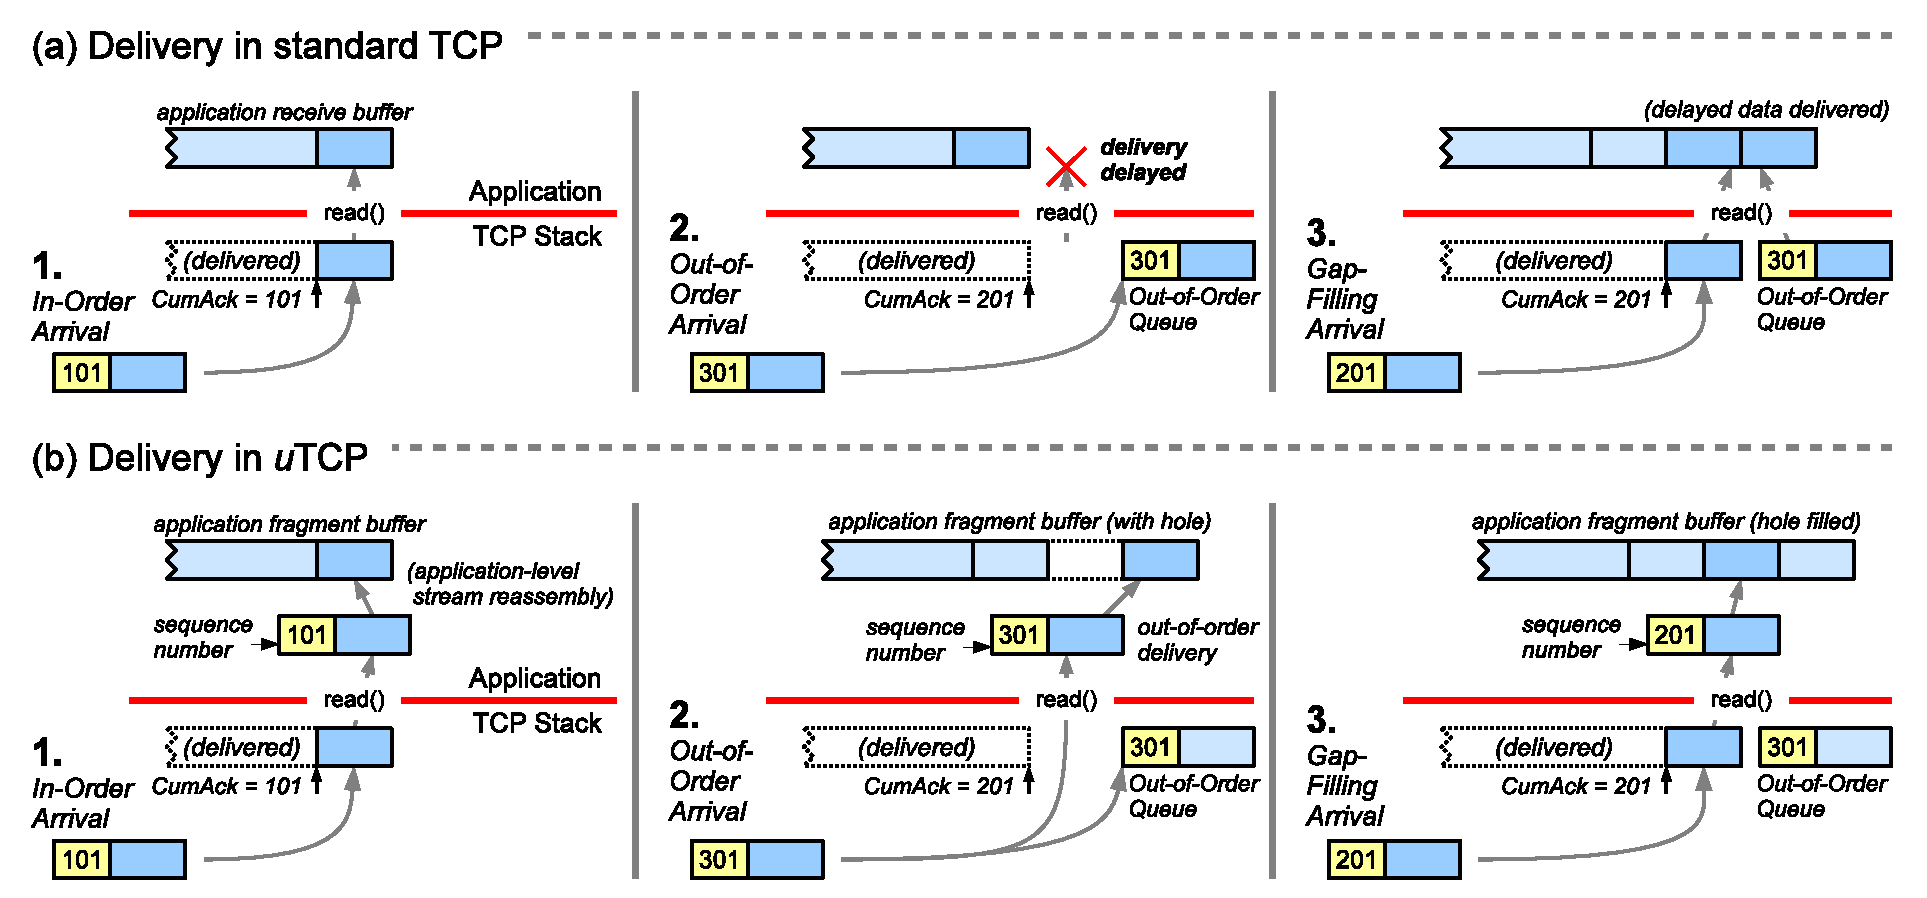
\includegraphics[width=0.99\textwidth]{figures/utcpdelivery.eps}
\caption{
Delivery behavior of (a) standard TCP, and (b) \utcp,
upon receipt of in-order and out-of-order segments.
(taken from~\cite{nowlan12fitting})}
\label{f:utcpdelivery}
\end{figure}

Figure~\ref{f:utcpdelivery} illustrates \utcp's receive-side behavior,
in a simple scenario
where three TCP segments arrive in succession:
first an in-order segment, then an out-of-order segment,
and finally a segment filling the gap between the first two.
With \utcp,
the application receives each segment as soon as it arrives,
along with the sequence number information it needs to reconstruct
a complete internal view of
whichever fragments of the TCP stream have arrived.

\subsubsection{\utcp: Sender-Side Modifications}
While \utcp's receiver-side enhancements
address the ``latency tax''
on segments waiting in TCP's reordering buffer,
TCP's sender-side queue can also introduce latency,
as segments the application has already written to a TCP socket---%
and hence ``committed'' to the network---%
wait until TCP's flow and congestion control
allow their transmission.
Many applications can benefit from the ability to ``late-bind''
their decision on {\em what} to send until the last possible moment,
and also from being able to transmit a message of higher priority
that bypasses any lower priority messages in the sender-side queue.

A \utcp sender allows a sending application
to specify a tag with each application write,
which the \utcp sender currently
interprets as a priority level.
Instead of unconditionally placing the newly-written data
at the tail of the send queue as TCP normally would,
\utcp{} {\em inserts} the newly-written data into the send queue
just {\em before} any lower-priority data
in the send queue not yet transmitted.

With these modifications to a TCP stack,
none of which require changes to the TCP wire-format,
\utcp offers an interface which,
while not convenient for applications, 
is powerful.
In the next Section,
we discuss how we build a userspace library that uses this interface
that provides a simple unordered delivery service,
unordered delivery of encrypted messages,
and logically separate data streams 
within a single \utcp connection.

\subsubsection{Datagrams atop \utcp}
\label{sec:dgrams_utcp}

Applications built on datagram substrates such as UDP
generally assume the underlying layer preserves datagram boundaries.
TCP's stream-oriented semantics do not preserve
any application-relevant frame boundaries within a stream, however.
Both the TCP sender and network middleboxes can and do
coalesce TCP segments or re-segment TCP streams
in unpredictable ways~\cite{honda2011still}.

Atop \utcp,
a userspace library can reconstruct contiguous fragments 
in the received data stream
using the metadata sequence number information 
that \utcp passes along at the receiver.
However,
providing unordered message delivery service atop \utcp
requires delimiting application messages in the bytestream.
While record delimiting is commonly done
by application protocols such as HTTP, SIP, and many others,
a key property that we require to provide a true unordered delivery service
is that a receiver must be able to extract a given message 
independently of other messages.
That is, 
as soon as a complete message is received,
the message delimiting mechanism must
allow for extraction of the message from the bytestream fragment,
without relying on the receipt of earlier messages.

Minion implements self-delimiting messages in two ways:
\begin{enumerate}
    \item To encode application datagrams efficiently, 
    the userspace library employs 
    {\em Consistent-Overhead Byte Stuffing}, or
    COBS~\cite{cheshire97consistent}
    to delimit and extract messages.
    COBS is a binary encoding
    which eliminates {\em exactly} one byte value from a record's encoding
    with minimal bandwidth overhead.
    To encode an application record,
    COBS first scans the record for {\em runs}
    of contiguous marker-free data followed by exactly one marker byte.
    COBS then removes the trailing marker,
    instead {\em prepending} a non-marker byte indicating the run length.
    A special run-length value indicates a run of 254 bytes
    {\em not} followed by a marker in the original data,
    enabling COBS to divide arbitrary-length runs into 254-byte runs
    encoded into 255 bytes each,
    yielding a worst-case expansion of only 0.4\%.

    \item The userspace library 
    coaxes out-of-order delivery from
    the {\em existing} TCP-oriented TLS wire format,
    producing an encrypted datagram substrate
    indistinguishable on the wire from standard TLS connections.
    TLS~\cite{rfc5246} already breaks its communication into {\em records},
    encrypts and authenticates each record,
    and prepends a header
    for transmission on the underlying TCP stream.
    TLS was designed to decrypt records strictly in-order, however,
    creating challenges 
    which the userspace library overcomes~\cite{nowlan12fitting}.
    Run on port 443,
    our encrypted stream atop \utcp is indistinguishable from HTTPS---%
    regardless of whether the application actually uses HTTP headers,
    since the HTTP portion of HTTPS streams are TLS-encrypted anyway.
    Deployed this way,
    Minion effectively offers an end-to-end protected substrate
    in the ``HTTP as the new narrow waist'' philosophy~\cite{popa10http}.
\end{enumerate}

\subsection{Impact on Real Applications}

Minion's unordered delivery service 
benefits a number of applications;
we refer the reader to detailed discussion and experiments 
in~\cite{nowlan12fitting}.
Of these applications,
we briefly discuss how Minion fits within
ongoing efforts to develop a next-generation transport for the web,
such as SPDY\cite{spdy} and the Internet Engineering Task Force (IETF)'s 
HTTP/2.0 (httpbis) effort.
Developing a next-generation HTTP 
requires either submitting to TCP's latency tax
for backward compatibility,
as with SPDY's use of TLS/TCP,
or developing and deploying new transports atop UDP,
neither of which,
as we discussed earlier in this section,
is a satisfying alternative.

Minion bridges this gap 
and demonstrates that it is possible to obtain
unordered delivery from wire-compatible TCP and TLS streams
with surprisingly small changes to TCP stacks
and application-level code.
These protocols offer latency-sensitive applications
performance benefits comparable to UDP or DCCP,
with the compatibility benefits of TCP and TLS.
Without discounting the value of UDP and newer OS-level transports,
Minion offers a more conservative path toward
the performance benefits of unordered delivery,
which we expect to be useful to applications
that use TCP for a variety of pragmatic reasons.

%\subsection{Editorial Note}
%Some of the text and figures in this Section have been adapted from
%the following two publications:


%\section{A glimpse into future transport protocols}
%%%%%%%%%%%%%%%%%%%%%%%%%%%%%%%%%%%%%%%%%%%%

%\clearpage
\section{Future Directions}
\label{sec:future}

There are some interesting tasks left for traffic matrix
research. The various algorithms and techniques described
here could be improved, though in many cases the improvements may be
relatively incremental given the success of existing approaches. More
interest may be found in extending the ideas and techniques used here
to new domains, and to evolving Internet traffic.

There are a few obvious cases (and no doubt many less obvious cases
that we have not thought of), for instance: multicast traffic has not,
to our knowledge, been studied in this way. Multicast is interesting
because it violates the {\em traffic conservation} assumption that
lies underneath many techniques for estimation and modelling of
traffic matrices. We could imagine modelling it by considering the
``flow'' to be the traffic on a multicast group, from say, one source,
to a set of destinations, and then stacking a vector with these. The
routing matrices now include elements for every link used (no longer
following a single path). The traffic ``matrix'' could then be a
column vector of the traffic on each of these flows. So the idea of
multicast traffic can fit into the structure we have talked about
here, but appropriate models for performing tasks such as inference
do not seem to exist.

It would also be very interesting to understand the way that CDNs are
affecting network traffic. A step in this direction, although not directly
on traffic, but more on the discovery of the content hosts is \cite{Ager11CDN}.
A CDN's typical goal is to bring content
closer to the user, thereby reducing network traffic. However, that
explicitly violates the ``friction free'' assumption in most gravity
models, and introduces distance as something to be modelled.

That leads naturally to the consideration of global traffic. Almost all
studies of traffic have concentrated on a single network no larger
than the national scale. That may still be very large -- for example,
several studies looked at Tier 1 providers in the USA, which for some
time dominated Internet traffic. However, although large, it was still
relatively homogeneous traffic between people speaking much the same
language(s) from place to place in the network. When we consider the
Internet globally, we may see that there are language or cultural
clusters where large groupings of traffic are focussed.

On a large scale, time zones also play a significant role. Traffic
patterns show strong cyclic behaviour based on user activity, but such
activity is strongly dependent on the local time zone. If traffic is
flowing from user to user, then this can result in strong apparent
locality effects, simply because people in the same time zone are more
likely to be awake at the same time \cite{gerber:03}. 
 
While language and cultural focussing may be geographic in nature, it
might also be considered per network, and that leads to another topic
of some interest. Very few papers have tried to consider inter-AS
(also known as inter-domain) traffic in any detail. Exceptions are
Chang~\etal\cite{Chang05EmpiricalAS} (which presents suggestions for
estimating traffic based on models derived from business models and resulting
usage); Bharti~\etal\cite{Bharti10Invisible} (which considered
inference of hidden elements of this matrix using a subset of data),
Feldman~\etal\cite{Feldmann04Web} (which aimed to estimate a global
traffic matrix, but only in the limited domain of WWW traffic), and
Labovitz~\etal\cite{labovitz10:_inter_inter_domain_traff} (which
looked at inter-domain traffic from 110 network operators over a
two-year period, though not in the form of a matrix). Study of the
Internet's global traffic matrix is made difficult by the sheer scale
of the project: Labovitz~\etal studied 110 network operators over a
two-year period\footnote{To put this in context, there are tens of
  thousands of ASes in the Internet.} and to do so, collected over 200
Exabytes of data. Many network operators do not collect or store data
of the type required for such a study, and many more regard it as
proprietary or covered by privacy legislation with provisions such
that no researcher is ever likely to see it. So we can see that study
of the inter-domain matrix is likely to be a long-term, and rather
challenging project.

In addition, we know that the {\em traffic profile} (or mix of
applications) has changed fairly rapidly over time. It is likely this
trend will continue, and there are bound to be effects on traffic
patterns as a result. Peer-2-peer traffic significantly altered
traffic patterns when it appeared because it was more symmetric than
traditional (at the time) WWW traffic. However, in addition,
peer-2-peer applications have the potential to exploit locality
information to download from sources closer to the destination. This
could potentially change the ``no friction'' assumption in much the
same way that CDNs can, though in the early days it did not appear to
be the case \cite{gerber:03}. An example traffic matrix (drawn from
\cite{gerber:03}) showing normalised\footnote{The elements have been
  normalised by dividing each row by the row-sum, so that each element
  actually represents the probability that a packet enters the network
  at a given region $i$ will depart the network at region $j$.}
traffic between regions in a cable-network operator is given in
\autoref{tab:cable_tm}. The major deviation, in this data, from a pure
gravity model seemed to be time-zone differences.

\begin{table}[!h]
  \centering
  \begin{tabular}{r|rrrrrrrr}
    From/To & R1 & R2 & R3 & R4 & R5 & R6 & R7 & R8 \\
    \hline
    R1 & -     & 0.180 & 0.140 & 0.126 & 0.174 & 0.128 & 0.124 & 0.127 \\
    R2 & 0.172 & -     & 0.141 & 0.126 & 0.190 & 0.132 & 0.118 & 0.120 \\
    R3 & 0.132 & 0.120 & -     & 0.189 & 0.135 & 0.145 & 0.139 & 0.140 \\
    R4 & 0.107 & 0.111 & 0.182 & -     & 0.124 & 0.163 & 0.155 & 0.158 \\
    R5 & 0.161 & 0.180 & 0.136 & 0.132 & -     & 0.135 & 0.127 & 0.129 \\
    R6 & 0.107 & 0.108 & 0.145 & 0.155 & 0.125 & -     & 0.187 & 0.173 \\
    R7 & 0.107 & 0.106 & 0.137 & 0.157 & 0.127 & 0.182 & -     & 0.184 \\
    R8 & 0.109 & 0.111 & 0.127 & 0.161 & 0.128 & 0.178 & 0.185 & - \\
  \end{tabular}
  \caption{Normalised inter-regional traffic matrix from \cite{gerber:03}.}
  \label{tab:cable_tm}
\end{table}

% T = [
%  [ 0     , 0.180 , 0.140 , 0.126 , 0.174 , 0.128 , 0.124 , 0.127 ]
%  [ 0.172 , 0     , 0.141 , 0.126 , 0.190 , 0.132 , 0.118 , 0.120 ]
%  [ 0.132 , 0.120 , 0     , 0.189 , 0.135 , 0.145 , 0.139 , 0.140 ]
%  [ 0.107 , 0.111 , 0.182 , 0     , 0.124 , 0.163 , 0.155 , 0.158 ]
%  [ 0.161 , 0.180 , 0.136 , 0.132 , 0     , 0.135 , 0.127 , 0.129 ]
%  [ 0.107 , 0.108 , 0.145 , 0.155 , 0.125 , 0     , 0.187 , 0.173 ]
%  [ 0.107 , 0.106 , 0.137 , 0.157 , 0.127 , 0.182 , 0     , 0.184 ]
%  [ 0.109 , 0.111 , 0.127 , 0.161 , 0.128 , 0.178 , 0.185 , 0 ]
% ]

New traffic classes may change traffic matrices in the future, and
modelling these will be interesting. On the other side, applications
such as anomaly detection are likely to remain interesting due to
their immediate benefits to operators, but the most overlooked task is
traffic matrix synthesis. As mentioned in the previous section, the
lack of real world traffic matrix datasets motivates the use of
artificial traffic matrices to provide some degree of approximation in
network traffic planning, provisioning and engineering tasks.  It is
an important area to concentrate on, considering its usefulness to
network operators.

%Synthesis means generating artificial traffic matrices, typically for
%use in simulations. There are only, to our knowledge, two papers
%\cite{Nucci05TMSynth,Roughan05GravSynth} on synthesising Internet
%traffic matrices, but there are already quite a few where synthetic
%traffic matrices were used, and this demand for such matrices will
%continue.
%
%Synthesis is not demanding in some ways. Traffic matrices are usually
%relatively small (compared to other types of traffic data), when
%measured at a reasonable level of aggregation and time scale. However,
%in other ways these matrices are quite challenging. For instance:
%\begin{itemize}
%
%\item we have few sets of traffic matrix data, and even fewer that are
%  public, and somehow need to use these to estimate properties of
%  these complex, high-dimensional objects;
%
%\item there is a real relationship between topology and traffic
%  (although we would like a traffic matrix to be invariant to the
%  topology, there are clear cases where, particularly IE matrices are
%  not);
%
%\item traffic matrices come in a wide variety of types (at different
%  levels of aggregation, for particular applications and so on) and it
%  is unlikely that one model fits all; and 
%
%\item there are a number of conflicting goals in synthesis, \eg~to
%  generate variability, but well ``matched'' to real traffic
%  matrices. 
%
%\end{itemize}
%However, there is considerable hope that progress can be made in terms
%of generating synthetic matrices, both for green-fields network design
%\cite{Kowalski95TeleModel}, and for simulation in general. 
%
%The major use of synthesis is in simulation. In many cases a traffic
%matrix is enough for a simulation, but in others, we need to translate
%this into packets (or at least connections). The analogue in
%transportation modelling is often called a {\em micro-simulation}
%model. Here, the problem becomes one of taking a {\em demand} matrix
%(remember, most of the work here is related to traffic, not demand), and
%translating this into carried load. We know how to do that (using
%simulation tools such as \verb|ns|) but doing it efficiently is
%difficult. One paper \cite{sommers11:_effic} starts to tackle this
%problem, but as in the work of transportation modelling, there is
%considerable scope for advanced scalable micro-simulation of traffic.
%
%Another use for synthetic traffic matrices is in the further task of
%synthetic topology generation, but we shall leave discussion of this
%topic to another section of this book.


\section{Conclusion}\label{section:conclusion}
%%%%%%%%%%%%%%%%%

%\ed{A one page conclusion.} 
%Something on evolution of transport
%Something on Middleboxes
%Something on MPTCP
%Something on Minion
%One paragraph on the future

The Transport Layer in the Internet evolved for nearly two decades,
but it has been stuck for over a decade now.
A proliferation of middleboxes in the Internet,
devices in the network that look past the IP header,
has shifted the waist of the Internet hourglass 
upward from IP
to include UDP and TCP,
the legacy workhorses of the Internet.
While popular for many
different reasons, 
middleboxes thus deviate from the Internet’s
end-to-end design, creating large deployment
“black-holes”---singularities where legacy transports get through, but
any new transport technology or protocol fails,
severely limiting transport protocol evolution.
The fallout of this ossification
is that new transport protocols,
such as SCTP and DCCP,
that were developed to offer much needed 
richer end-to-end services to applications,
have had trouble getting deployed since they require changes 
to extant middleboxes.

Multipath TCP is perhaps the most significant change to TCP in the past twenty
years. It allows existing TCP applications to achieve better
performance and robustness over today's networks, and it has been
standardized at the IETF. The Linux kernel implementation shows that
these benefits can be obtained in practice.  However, as with any
change to TCP, the deployment bar for Multipath TCP is very high: only
time will tell whether the benefits it brings will outweigh the added
complexity it brings in the end-host stacks.

The design of Multipath TCP has been a lengthy, painful process that took around five
years. Most of the difficulty came from the need to support existing middlebox
behaviors, while offering the exact same service to applications as TCP. Although
the design space seemed wide open in the beginning, in the end we were \emph{just} able
to evolve TCP this way: for many of the design choices there was only one viable option
that could be used. When the next major TCP extension is designed in a network with even more
middleboxes, will we, as a community, be as lucky?

A pragmatic answer to the inability to deploy new transport protocols
is Minion. It allows deploying new transport services 
by being backward compatible with middleboxes by encapsulating new protocols inside TCP.
Minion demonstrates that it is possible to obtain
unordered delivery and multistreaming
from wire-compatible TCP and TLS streams
with surprisingly small changes to TCP stacks
and application-level code.
Minion offers a path toward
the performance benefits of unordered delivery,
which we expect to be useful to applications
that use TCP for a variety of pragmatic reasons.

%Minion is just the latest in an ever-growing encapsulation war that 
%has engulfed end-hosts and network providers for years on end. 
Early in the Internet's history,
all IP packets could travel freely through the Internet, as IP was the narrow waist of
the protocol stack. 
Eventually, 
apps started using UDP and TCP exclusively,
and some, such as Skype, used them adaptively,
probably due to security concerns
in addition to the increasing proliferation of middleboxes that allowed only UDP and TCP through.
As a result, UDP and TCP over IP were then perceived to constitute the new waist of the Internet.
(We'll note that HTTP has also recently
been suggested as the new waist~\cite{popa10http}.) 
%UDP is not that great getting through newer firewalls either, so TCP is the new narrow
%waist, or even HTTP as recently proposed. 

Our observation is that
whatever the new waist is,
middleboxes will embrace it and optimize for it: 
if MPTCP and/or Minion become popular, 
it is likely that middleboxes will be devised that understand these protocols
to optimize for the most successful use-case of these protocols
and to help protect any vulnerable applications using them.
One immediate answer from an application would be to
use the encrypted communication proposed in Minion---%
but actively hiding information from a network operator
can potentially encourage the network operator
to embed middleboxes that intercept encrypted connections,
effectively mounting man-in-the-middle attacks
to control traffic over their network,
as is already being done in several corporate firewalls~\cite{marko10using}.
%a potential serious security breach, and many ISPs
%may either drop traffic or require their customers to ``install'' keys in the 
%browser that effectively allow middleboxes to become a man-in-the-middle of the TLS connection. 
To bypass these middleboxes,
new applications may encapsulate their data {\em even} deeper,
leading to a vicious circle resembling an ``arms race'' for control
over network use.
% them looking even deeper in the packets. As we can see, 
%this is a vicious circle that no-one can ever win.

This ``arms race'' is a symptom of a fundamental tussle between
end-hosts and the network: end-hosts will always want to deploy new
applications and services, while the network will always want to allow and optimize only
existing ones~\cite{tussle}.
To break out of this vicious circle,
we propose that
end-hosts and the network must co-operate,
and that they must build cooperation into their protocols.
Designing and providing protocols and incentives for this cooperation may hold the key to creating a
truly evolvable transport (and Internet) architecture.



%\bibliographystyle{plain}

% Define style for bibtex bibliography
\bibliographystyle{../acm}
\bibliography{ebook,rfc}

\appendix

\section{Exercises}
%%%%%%%%%%%%%%%%

This appendix contains a few exercises on the evolution of transport protocols and their interactions with middleboxes.

\subsection{Transport protocols}

\begin{enumerate}

\item TCP provides a reliable transport service. Assuming that you control the two endpoints of a connection, how would you modify the TCP protocol to provide an unreliable service ? Explore two variants of such a transport service :
  \begin{itemize}
  \item an unreliable bytestream where bytes can be corrupted but where there are no losses
  \item an unreliable bytestream that prevents data corruption but can deliver holes in the bytestream
  \end{itemize}

\item Same question as above, but for SCTP.

\item TCP provides a connection-oriented bytestream service. How would you modify TCP to support a message-oriented service. Consider two variants of this service :
 \begin{itemize}
    \item A connection-oriented message-mode service that supports only small messages, i.e. all messages are smaller than one segment.
    \item A connection-oriented message-mode service that supports any message length. 
 \end{itemize}

\item The large windows extension for TCP defined in \cite{rfc1323} uses the \texttt{WScale} option to negotiate a scaling factor which is valid for the entire duration of the connection. Propose another method to transport a larger window by using a new type of option inside each segment. What are the advantages/drawbacks of this approach compared to \cite{rfc1323} assuming that there are no middleboxes ?

\item One of the issues that limits the extensibility of TCP is the limited amount of space to encode TCP options. This limited space is particularly penalizing in the SYN segment. Explore two possible ways of reducing the consumption of precious TCP option-space
\begin{itemize}
\item Define a new option that packs several related options in a smaller option. For example try to combine SACK with Timestamp and Window scale in a small option for the SYN segment. 
\item Define a compression scheme that allows to pack TCP options in fewer bytes. The utilisation of this compression scheme would of course need to be negotiated during the three way handshake.
\end{itemize}



\end{enumerate}

\subsection{Middleboxes}

Middleboxes may perform various changes and checks on the packets that they process.  Testing  real middleboxes can be difficult because it involves installing complex and sometimes costly devices. However, getting an understanding of the interactions between middleboxes and transport protocols can be useful for protocol designers. 

A first approach to understand the impact of middleboxes on transport protocols is to emulate the interference caused by middleboxes.This can be performed by using \texttt{click} \cite{Kohler_click:2000} elements that emulate the operation of middleboxes \cite{Hesmans_click:2013} : 
\begin{itemize}
\item \texttt{ChangeSeqElement} changes the sequence number in the TCP header of processed segments to model a firewall that randomises sequence numbers
\item \texttt{RemoveTCPOptionElement} selectively removes a chosen option from processed TCP segments
\item \texttt{SegSplitElement} selectively splits a TCP segment in two different segments and copies the options in one or both segments
\item \texttt{SegCoalElement} selectively coalesces consecutive segments and uses the TCP option from the first/second segment for the coalesced one
\end{itemize}

Using some of these \texttt{click} elements, perform the following tests with one TCP implementation. 

\begin{enumerate}

\item Using a TCP implementation that supports the timestamp option defined in \cite{rfc1323} evaluate the effect of removing this option in the \texttt{SYN}, \texttt{SYN+ACK} or regular TCP segments with the \texttt{RemoveTCPOptionElement} \texttt{click} element.

\item Using a TCP implementation that supports the selective acknowledgement option defined in \cite{rfc2018} predict the effect randomizing the sequence number in the TCP header without updating anything in this option as done by some firewalls. Use the \texttt{ChangeSeqElement} \texttt{click} element to experimentally verify your answer. Instead of using random sequence numbers, evaluate the impact of logarithmically increasing/decreasing the sequence numbers (i.e. +10, +100, +1000, +1000, \ldots)

\item Recent TCP implementations support the large windows extension defined in \cite{rfc1323}. This extension uses the \texttt{WScale} option in the \texttt{SYN} and \texttt{SYN+ACK} segments. Evaluate the impact of removing this option in one of these segments with the \texttt{RemoveTCPOptionElement} element. For the experiments, try to force the utilisation of a large receive window by configuring your TCP stack.

\item Some middleboxes split or coalesce segments. Considering Multipath TCP, discuss the impact of splitting and coalescing segments on the correct operation of the protocol. Use the Multipath TCP implementation in the Linux kernel and the \texttt{SegCoalElement} and \texttt{SegSplitElement} \texttt{click} elements to experimentally verify your answer.

%\item Using the Multipath TCP implementation in the Linux kernel and one of the above mentioned \texttt{click} elements, 


\item The extensibility of SCTP depends on the utilisation of chunks. Consider an SCTP-aware middlebox that recognizes the standard SCTP chunks but drops the new ones. Consider for example the partial-reliability extension defined in \cite{rfc3758}. Develop a \texttt{click} element that allows to selectively remove a chunk from processed segments and evaluate experimentally its impact on SCTP.

\end{enumerate}

Another way to evaluate middleboxes is to try to infer their presence in a network by sending probe packets. This is the approach used by Michio Honda and his colleagues in \cite{honda2011still}. However, the TCPExposure software requires the utilisation of a special server and thus only allows to probe the path towards this particular server. An alternative is to use \texttt{tracebox} \cite{Detal_Tracebox:2013}. \texttt{tracebox} is an extension to the popular \texttt{traceroute} tool that allows to detect middleboxes on (almost) any path. \texttt{tracebox} sends TCP and UDP segments inside IP packets that have different Time-To-Live values like \texttt{traceroute}. When an IPv4 router receives an IPv4 packet whose TTL is going to expire, it returns an ICMPv4 \emph{Time Exceeded} packet that contains the offending packet. Older routers return in the ICMP the IP header of the original packet and the first 64 bits of the payload of this packet. When the packet contains a TCP segment, these first 64 bits correspond to the source and destination ports and the sequence number. However, recent measurements show that a large fraction of IP routers in the Internet, notably in the core, comply with \cite{rfc1812} and thus return the complete original packet. \texttt{tracebox} compares the packet returned inside the ICMP message with the original one to detect any modification performed by middleboxes. All the packets sent and received by \texttt{tracebox} are recorded as a libpcap file that can be easily processed by using \texttt{tcpdump} or \texttt{wireshark}.


\begin{enumerate}

\item Use \texttt{tracebox} to detect whether the TCP sequence numbers of the segments that your host sends are modified by intermediate firewalls or proxies.

\item Use \texttt{tracebox} behind a Network Address Translator to see whether \texttt{tracebox} is able to detect the modifications performed by the NAT. Try with TCP, UDP and regular IP packets to see whether the results vary with the protocol. Analyse the collected packet traces.

\item Some firewalls and middleboxes change the \texttt{MSS} option in the \texttt{SYN} segments that they process. Can you explain a possible reason for this change ? Use \texttt{tracebox} to verify whether there is a middlebox that performs this change inside your network.

\item Use \texttt{tracebox} to detect whether the middleboxes that are deployed in your network allow new TCP options, such as the ones used by Multipath TCP, to pass through.

\item Extend \texttt{tracebox} so that it supports the transmission of SCTP segments containing various types of chunks.


\end{enumerate}


\subsection{Multipath TCP}

Although Multipath TCP is a relatively young extension to TCP, it is already possible to perform interesting experiments and simulations with it. The following resources can be useful to experiment with Multipath TCP :

\begin{itemize}
\item \url{http://www.multipath-tcp.org} provides an implementation of Multipath TCP in the Linux kernel with complete source code and binary packages. This implementation covers most of \cite{rfc6824} and supports the coupled congestion control \cite{rfc6356} and OLIA \cite{olia}. Mininet and netkit images containing the Multipath TCP kernel are available from the above website.
\item \url{http://caia.swin.edu.au/urp/newtcp/mptcp/} provides a kernel patch that enables Multipath TCP in the FreeBSD-10.x kernel. This implementation only supports a subset of \cite{rfc6824}
\item The \texttt{ns-3} network simulator\footnote{See \url{http://www.nsnam.org/}.} contains two forms of support for Multipath TCP. The first one is by using a Multipath TCP model\footnote{See \url{https://code.google.com/p/mptcp-ns3/}}. The second is by executing a modified Linux kernel inside \texttt{ns-3}  by using Direct Code Execution\footnote{See \url{http://www.nsnam.org/projects/direct-code-execution/}}.

\end{itemize}

Most of the exercises below can be performed by using one of the above mentioned simulators or implementation. 

\begin{enumerate}

\item Several congestion control schemes have been proposed for Multipath TCP and some of them have been implemented. Compare the performance of the congestion control algorithms that your implementation supports. 

\item The Multipath TCP congestion control scheme was designed to move traffic away from congested paths. TCP detects congestion through losses. Devise an experiment using one of the above mentioned simulators/implementation to analyse the performance of Multipath TCP when losses occur.

\item The non-standard \texttt{TCP\_INFO} socket option\cite{Pfeiffer_Measuring:2007} in the Linux kernel allows to collect information about any active TCP connection. Develop an application that uses \texttt{TCP\_INFO} to study the evolution of the Multipath TCP congestion windows.


\item Using the Multipath TCP  Mininet or netkit image, experiment with Multipath TCP's fallback mechanism by using \texttt{ftp} to transfer files through a NAT that includes an application level gateway. Collect the packet trace and verify that the fallback works correctly.

\end{enumerate}



%\subsection {Minion}


%\ed{Any suggestion from Jana ?} 


\end{document}

